\chapter{Topological Cluster Data-MC Comparisons}\label{app:datamc}

In addition to the comparisons shown in the body of the work, the full set of comparisons between data and \gls{MC} for the topo-cluster variables used as inputs to the models presented are shown here. The number of topo-clusters is shown for unconverted photons in Figure~\ref{fig:dmc-u-ntopo}, and in Figure~\ref{fig:dmc-c-ntopo} for converted photons.

The distributions for $\sqrt{\lambda_{0}^2}$ and $\sqrt{r_{0}^2}$ for unconverted photons is shown in Section~\ref{ssec:yid-datamc}. The centroid depth, isolation, and \gls{EM} probability of the leading topo-cluster for unconverted photons are shown in Figures~\ref{fig:dmc-u-cl},~\ref{fig:dmc-u-iso}, and~\ref{fig:dmc-u-emp}, respectively. For converted photons, the leading topo-cluster $\sqrt{\lambda_{0}^2}$ is shown in Figure~\ref{fig:dmc-c-sl}, $\sqrt{r_{0}^2}$ is shown in Figure~\ref{fig:dmc-c-sr}, centroid depth is shown in Figure~\ref{fig:dmc-c-cl}, isolation is shown in Figure~\ref{fig:dmc-c-iso}, and \gls{EM} probability is shown in Figure~\ref{fig:dmc-c-emp}. Plots are binned according to the \pt and $\eta$ bins used in the photon ID menu.

In general, the \gls{MC} models the unconverted photons well, with the exception of the isolation, particularly in the most central bin and beyond the crack. For converted photons, $\sqrt{r_{0}^2}$ modeling differs between data and \gls{MC}, and isolation differs considerably, particularly in the most central bin. On average converted photons have more topo-clusters per photon object, meaning they suffer more from cluster splitting, which influences these effects.

\begin{figure}[!thp]
    \centering
    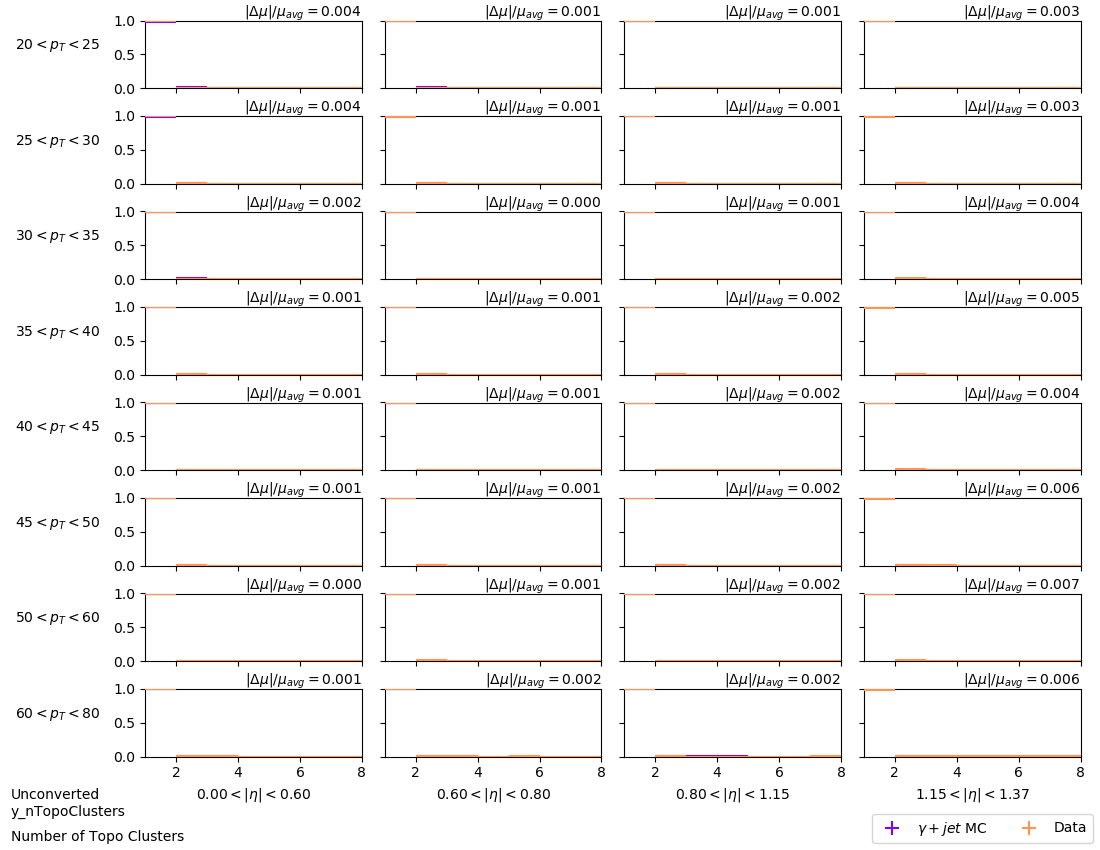
\includegraphics[width=.74\textwidth]{appendices/datamc_images/y_nTopoClusters_Unconverted_lowerEta.png}
    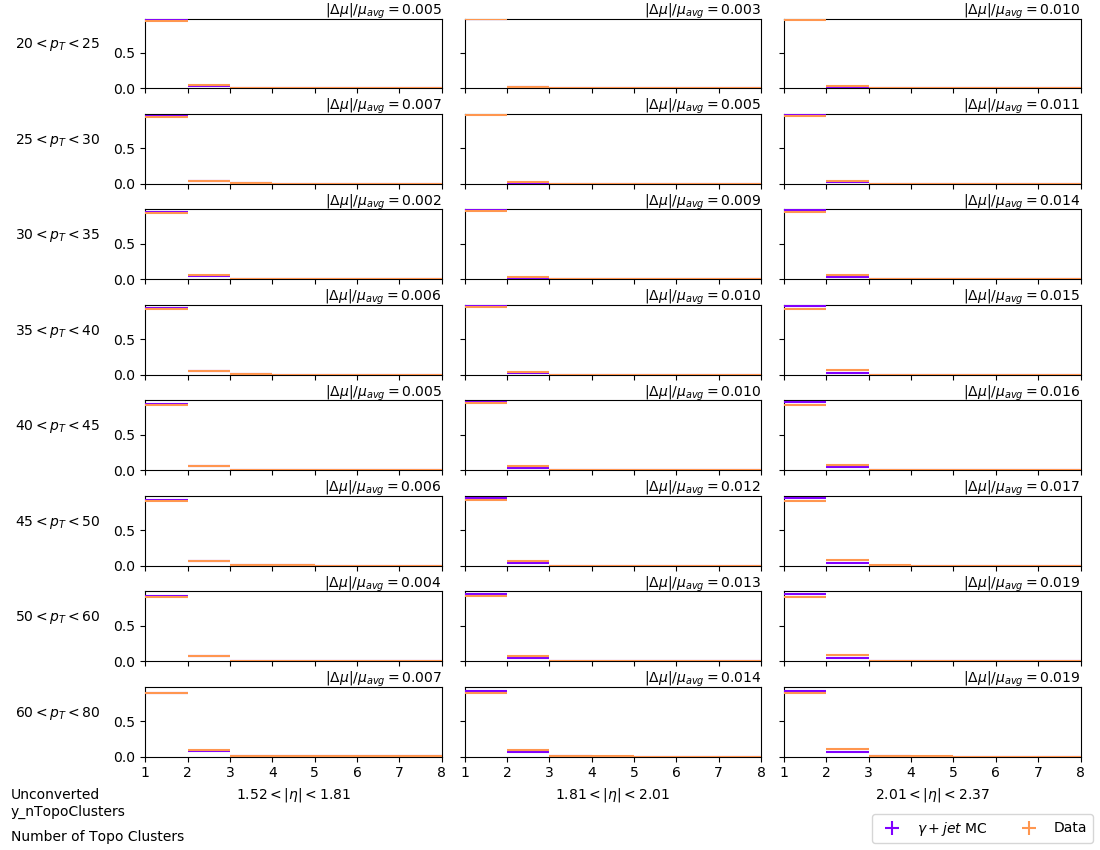
\includegraphics[width=.74\textwidth]{appendices/datamc_images/y_nTopoClusters_Unconverted_upperEta.png}
    \caption[Data-MC comparison of the number of topo-clusters for converted photons]{Data-MC comparison of the number of topo-clusters for converted photons. The current tight identification is applied to both samples, and the \gls{MC} requires truth-matched photons. The absolute difference of the distribution means normalized to their average mean, $|\Delta \mu|/\mu_{avg}|$ is shown.}
    \label{fig:dmc-u-ntopo}
\end{figure}
\begin{figure}[!thp]
    \centering
    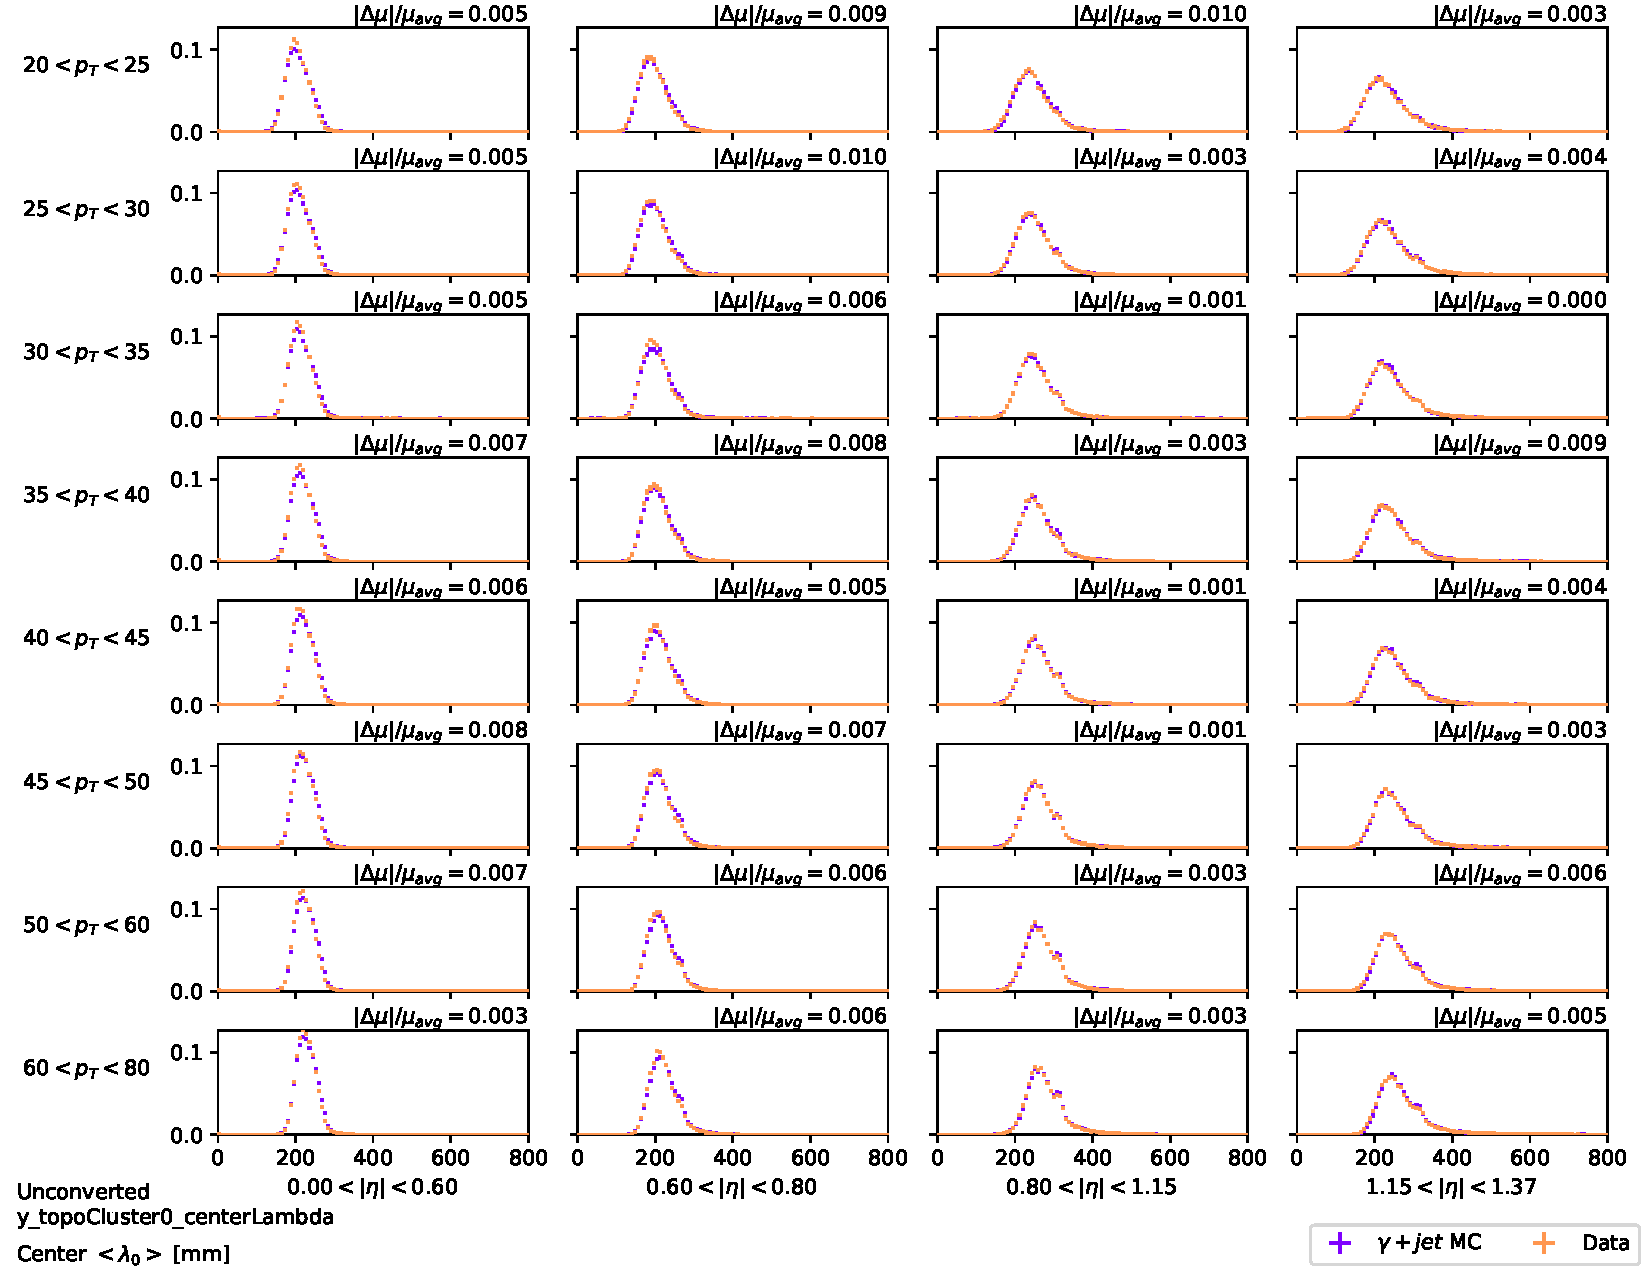
\includegraphics[width=.74\textwidth]{appendices/datamc_images/y_topoCluster0_centerLambda_Unconverted_lowerEta.pdf}
    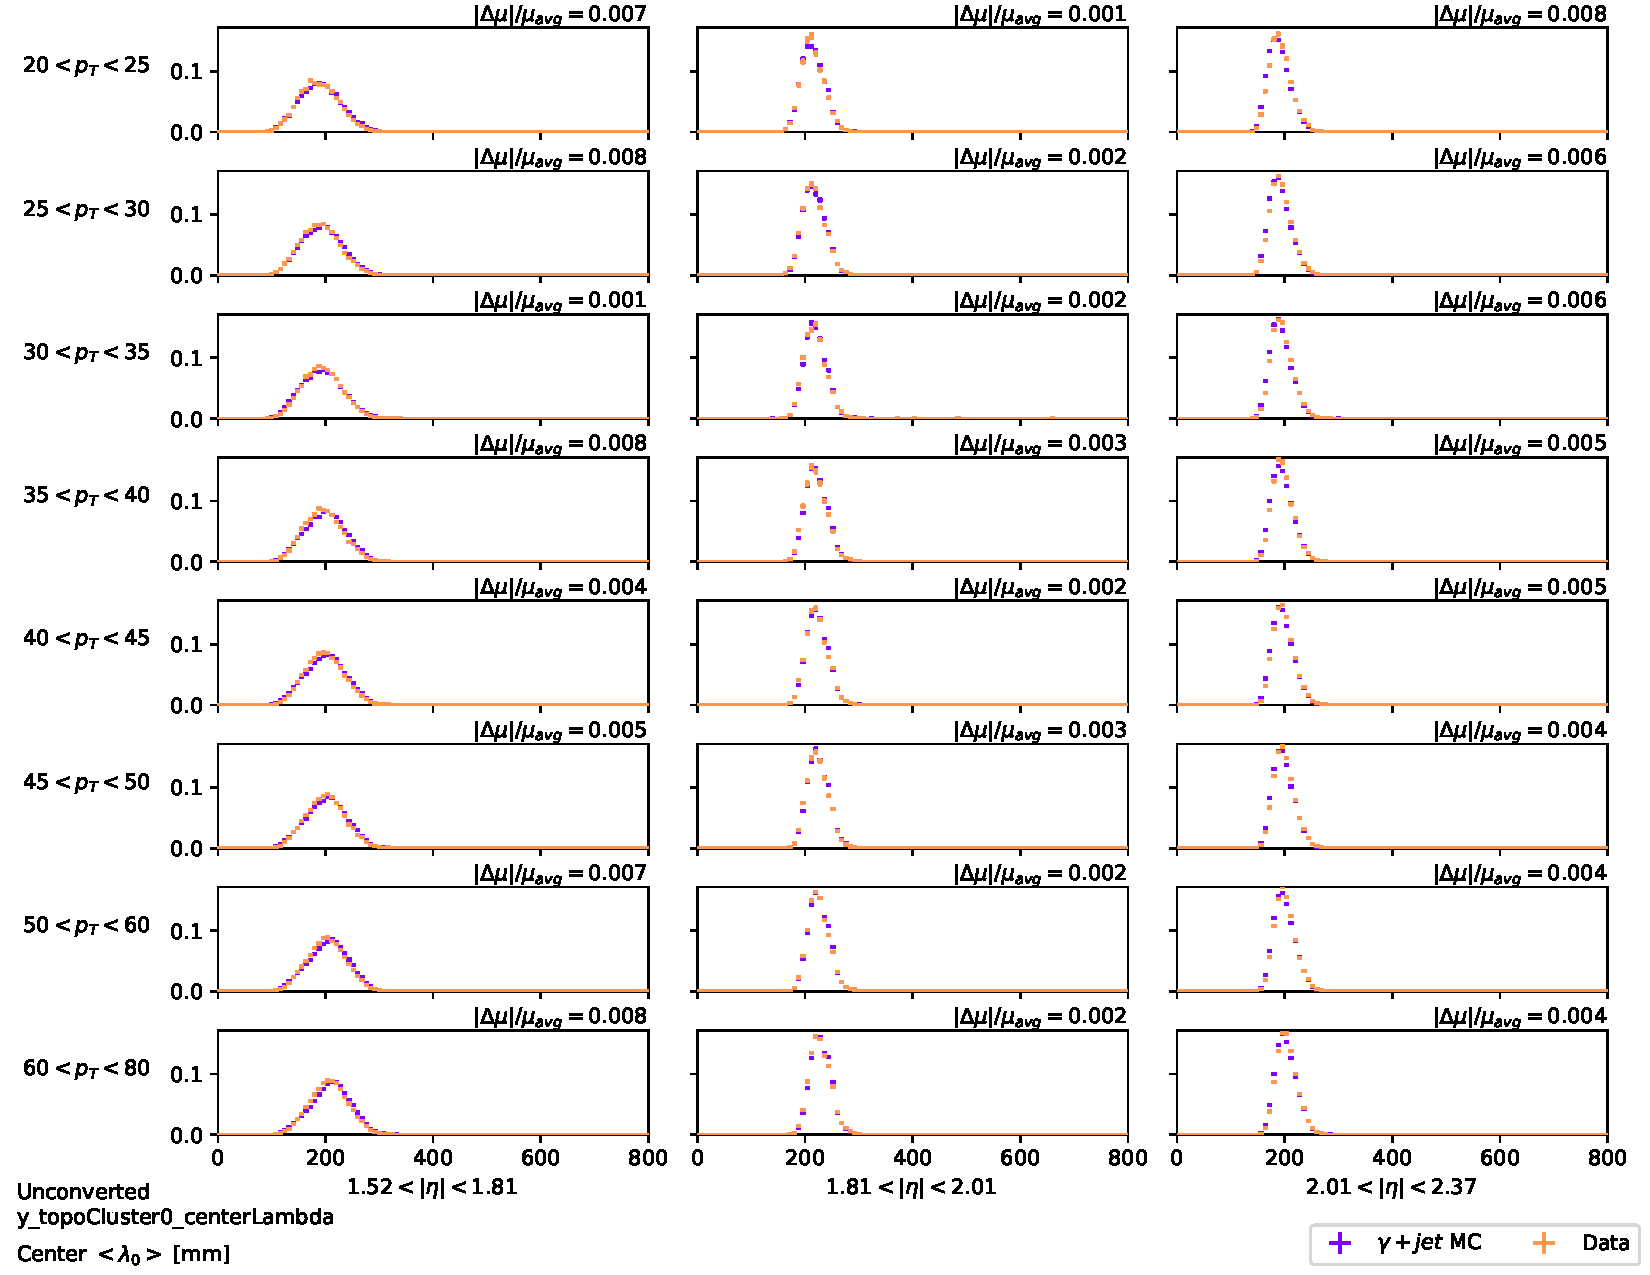
\includegraphics[width=.74\textwidth]{appendices/datamc_images/y_topoCluster0_centerLambda_Unconverted_upperEta.pdf}
    \caption[Data-MC comparison of the centroid depth of the leading topo-cluster (${<\lambda_{0}>}$) for unconverted photons]{Data-MC comparison of the centroid depth of the leading topo-cluster ($<\lambda_{0}>$) for unconverted photons. The current tight identification is applied to both samples, and the \gls{MC} requires truth-matched photons. The absolute difference of the distribution means normalized to their average mean, $|\Delta \mu|/\mu_{avg}|$ is shown.}
    \label{fig:dmc-u-cl}
\end{figure}

\begin{figure}[!thp]
    \centering
    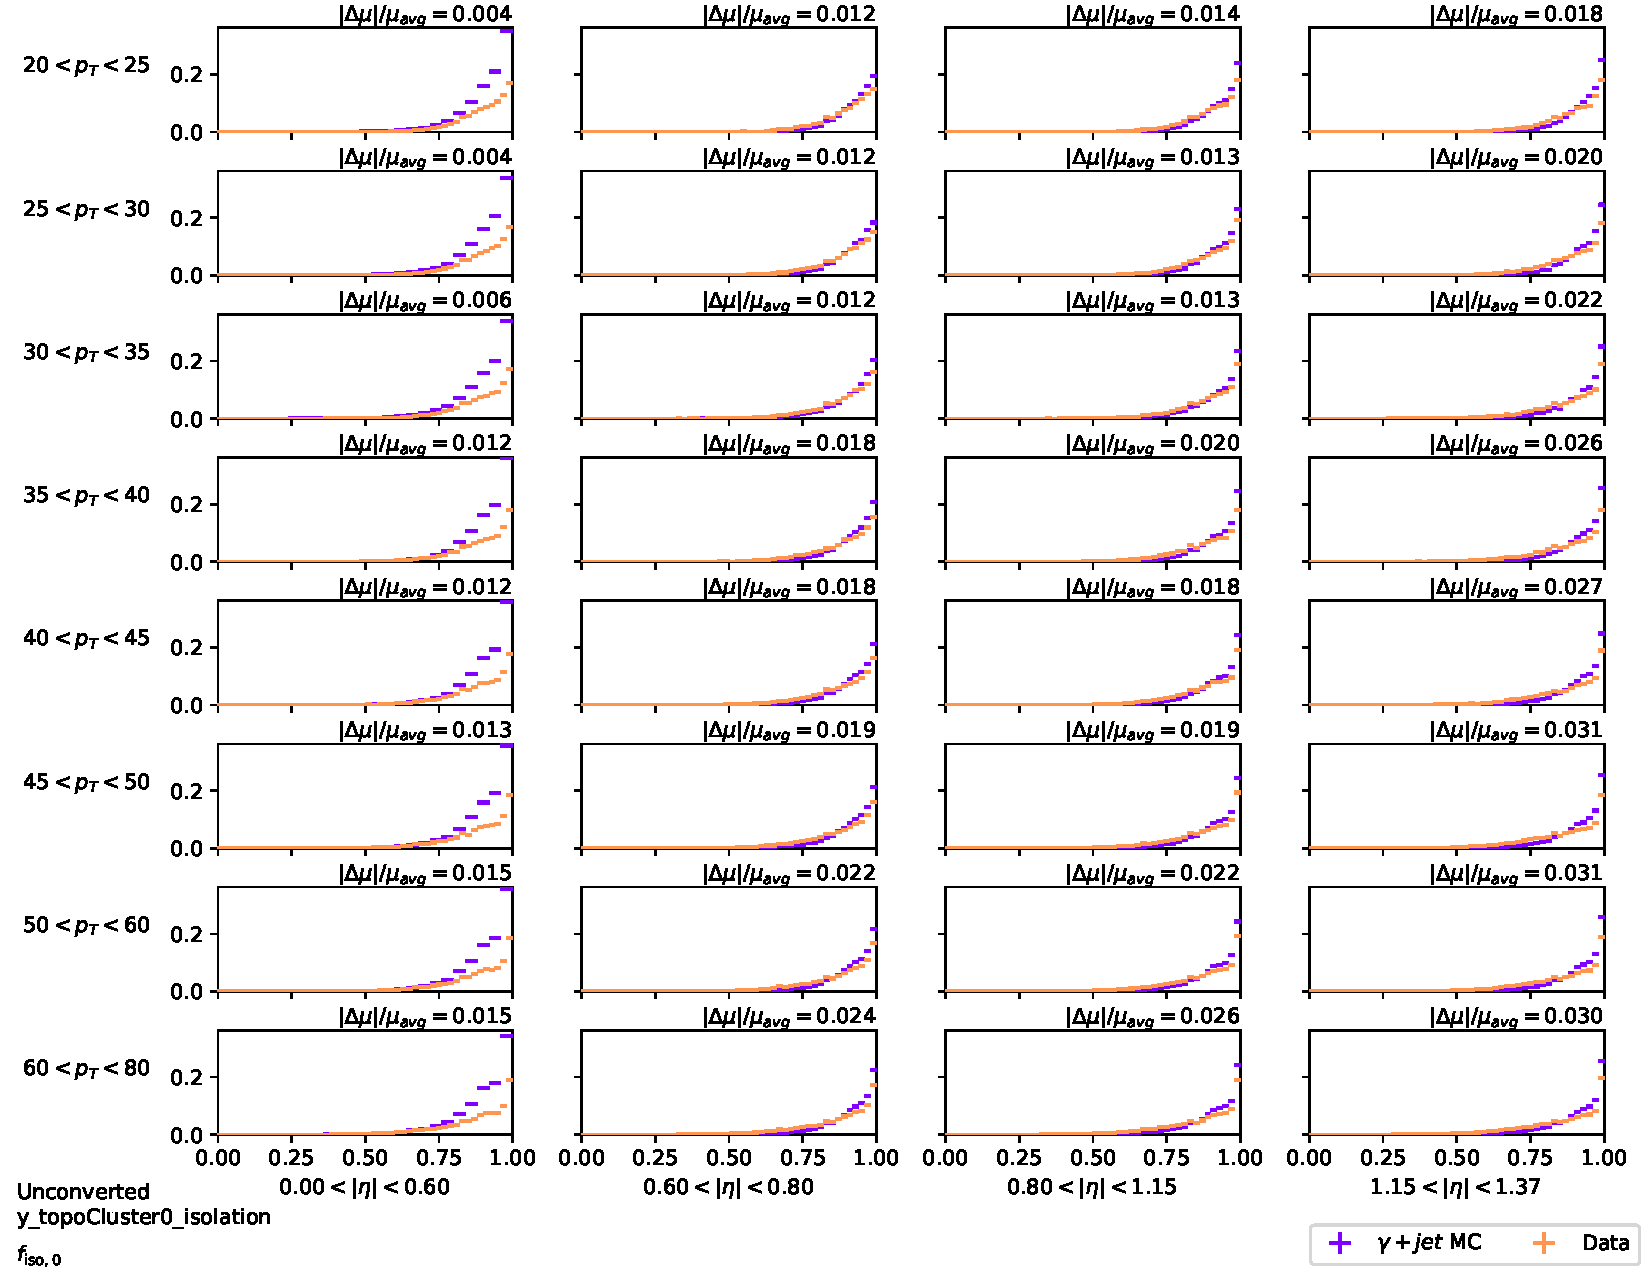
\includegraphics[width=.74\textwidth]{appendices/datamc_images/y_topoCluster0_isolation_Unconverted_lowerEta.pdf}
    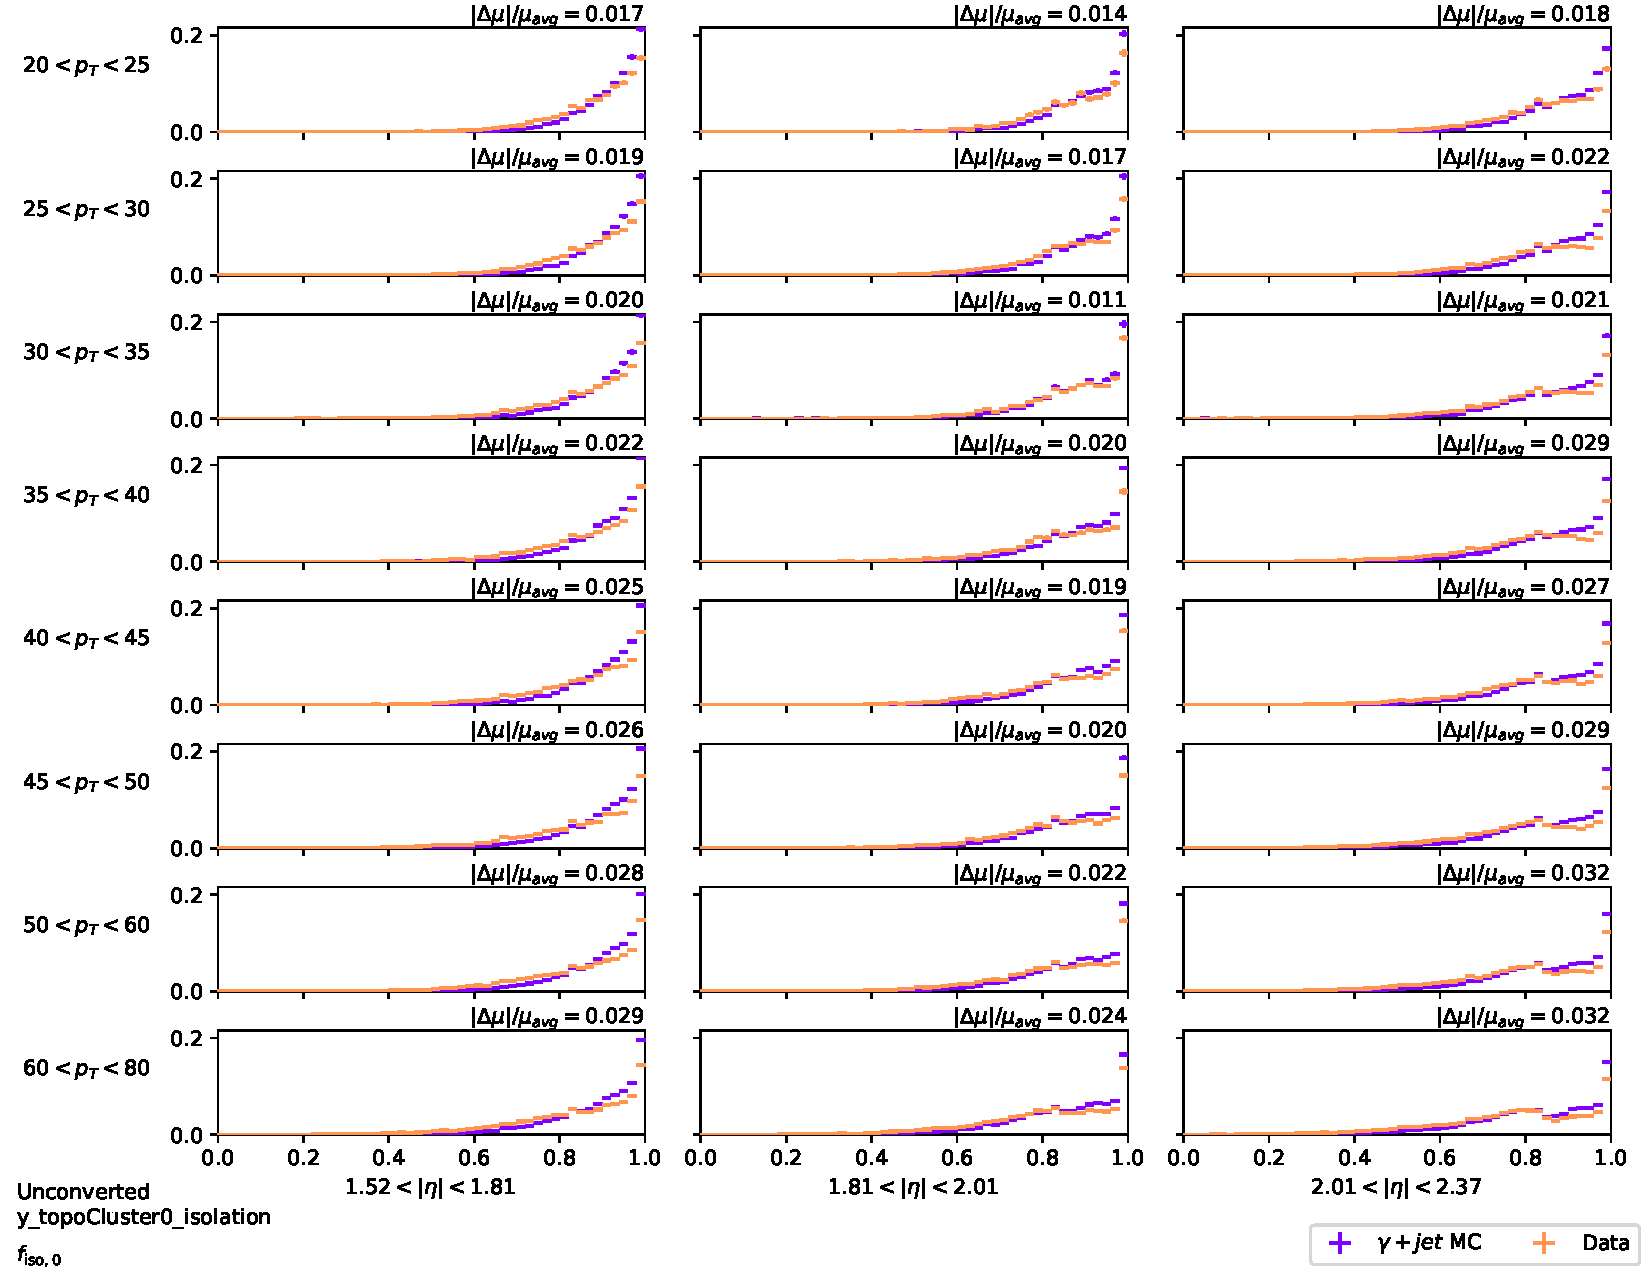
\includegraphics[width=.74\textwidth]{appendices/datamc_images/y_topoCluster0_isolation_Unconverted_upperEta.pdf}
    \caption[Data-MC comparison of the isolation of the leading topo-cluster ($f_{\text{iso}}$) for unconverted photons]{Data-MC comparison of the isolation of the leading topo-cluster ($f_{\text{iso}}$) for unconverted photons. The current tight identification is applied to both samples, and the \gls{MC} requires truth-matched photons. The absolute difference of the distribution means normalized to their average mean, $|\Delta \mu|/\mu_{avg}|$ is shown.}
    \label{fig:dmc-u-iso}
\end{figure}


\begin{figure}[!thp]
    \centering
    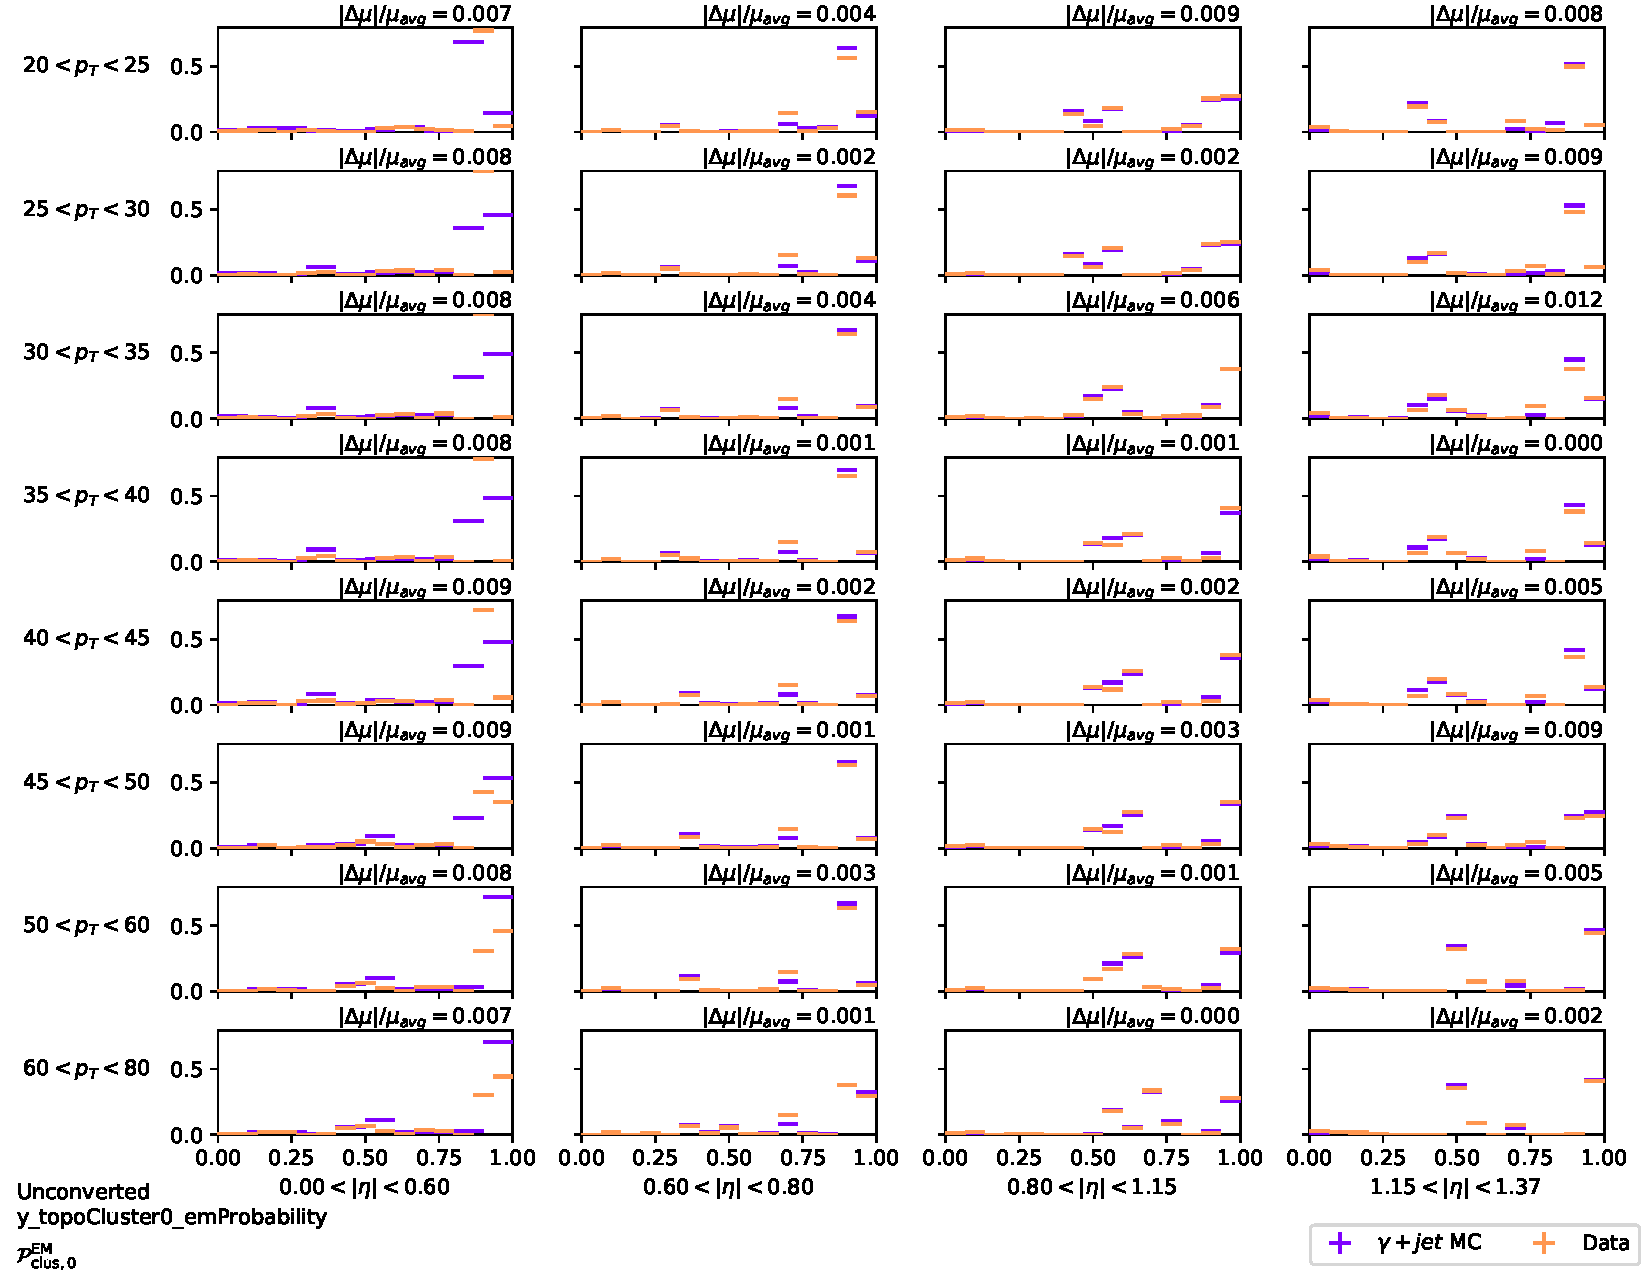
\includegraphics[width=.74\textwidth]{appendices/datamc_images/y_topoCluster0_emProbability_Unconverted_lowerEta.pdf}
    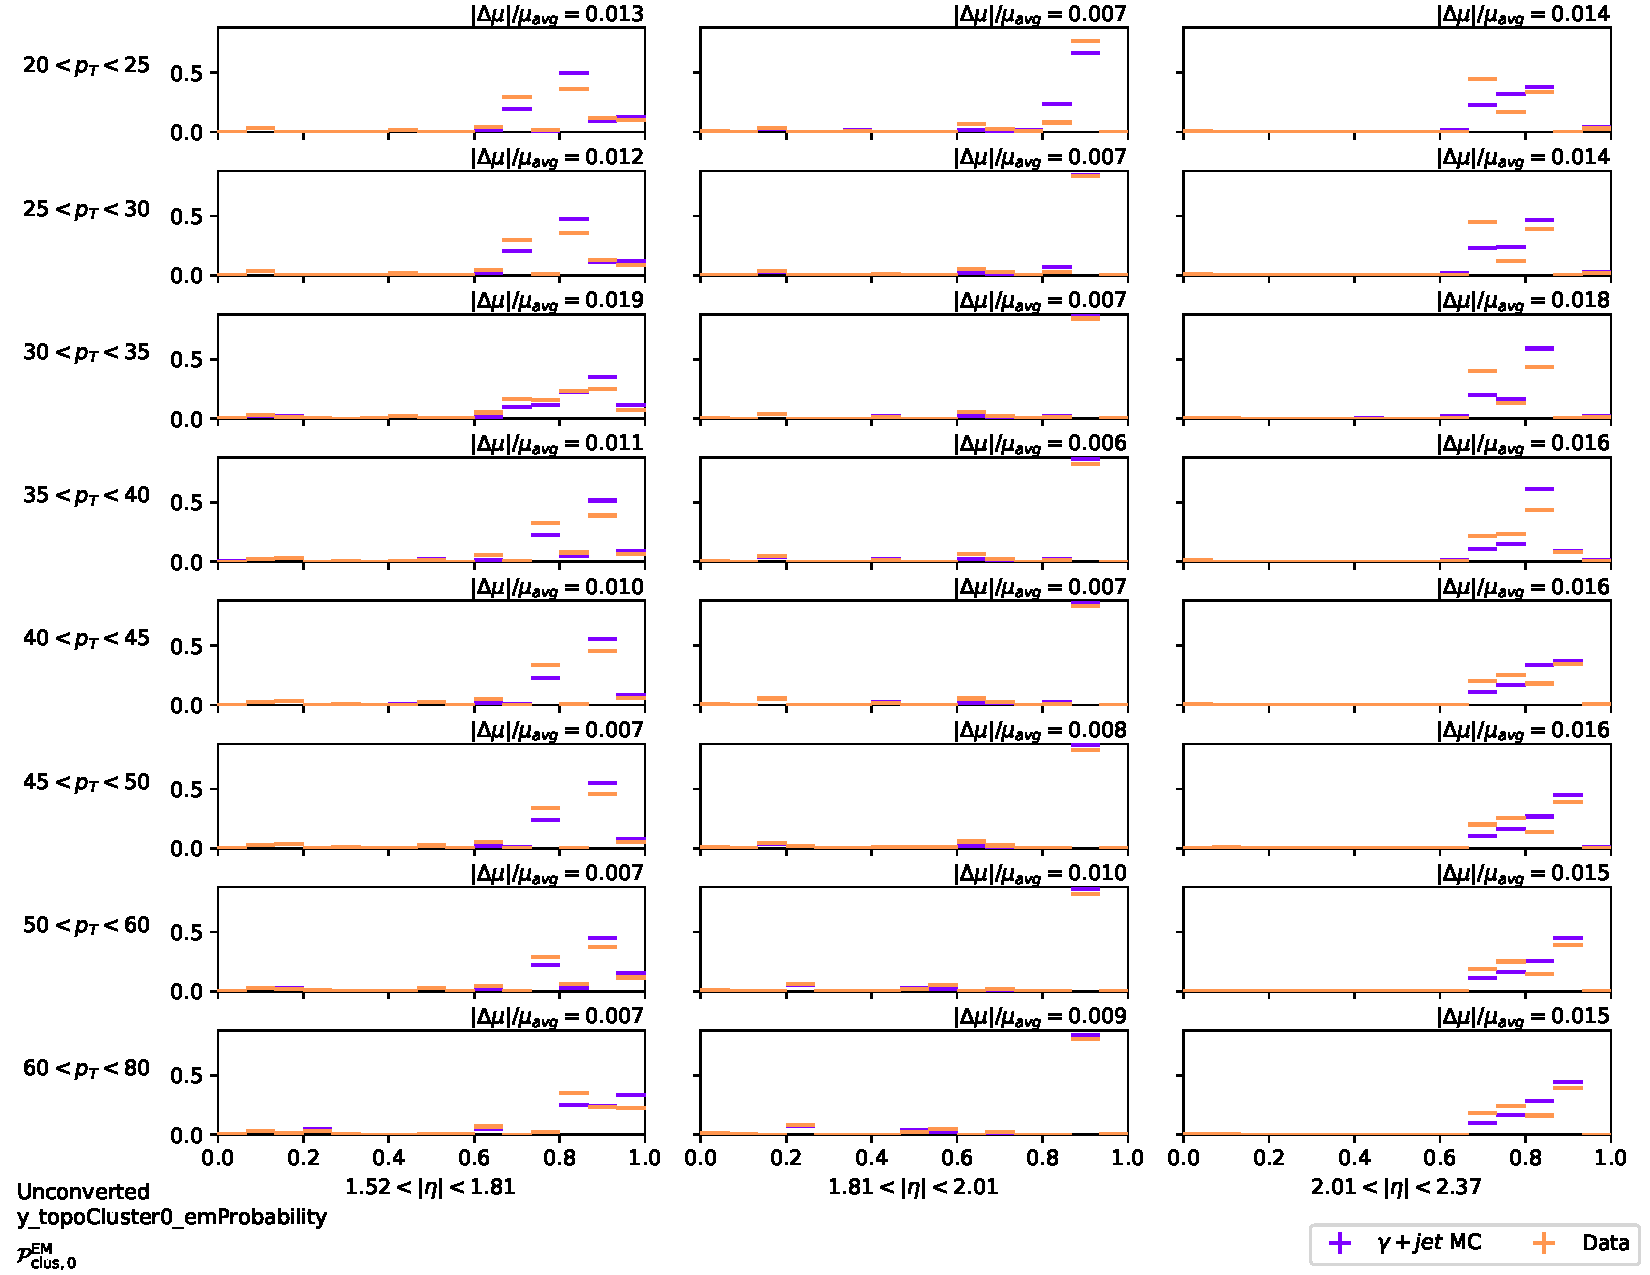
\includegraphics[width=.74\textwidth]{appendices/datamc_images/y_topoCluster0_emProbability_Unconverted_upperEta.pdf}
    \caption[Data-MC comparison of the \gls{EM} probability of the leading topo-cluster ($\mathcal{P}_{\text{clus}}^{\text{EM}}$) for unconverted photons]{Data-MC comparison of the \gls{EM} probability of the leading topo-cluster ($\mathcal{P}_{\text{clus}}^{\text{EM}}$) for unconverted photons. The current tight identification is applied to both samples, and the \gls{MC} requires truth-matched photons. The absolute difference of the distribution means normalized to their average mean, $|\Delta \mu|/\mu_{avg}|$ is shown.}
    \label{fig:dmc-u-emp}
\end{figure}




\begin{figure}[!thp]
    \centering
    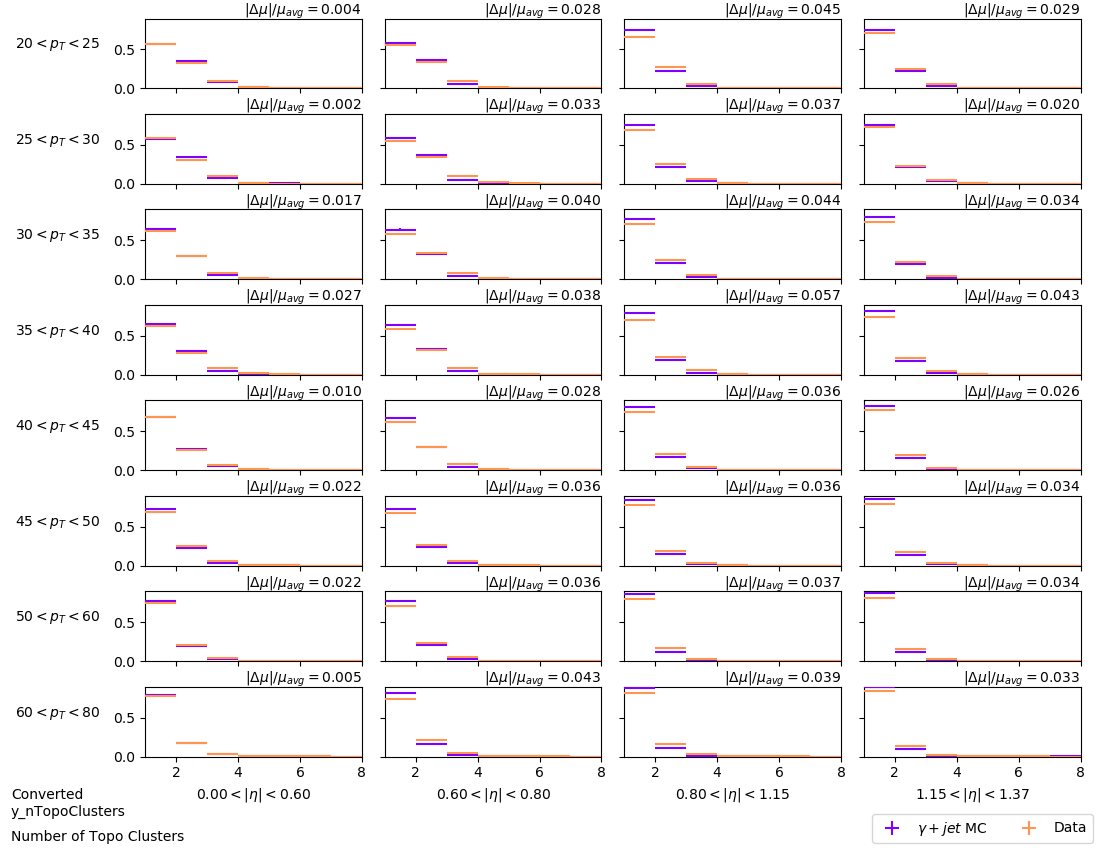
\includegraphics[width=.74\textwidth]{appendices/datamc_images/y_nTopoClusters_Converted_lowerEta.png}
    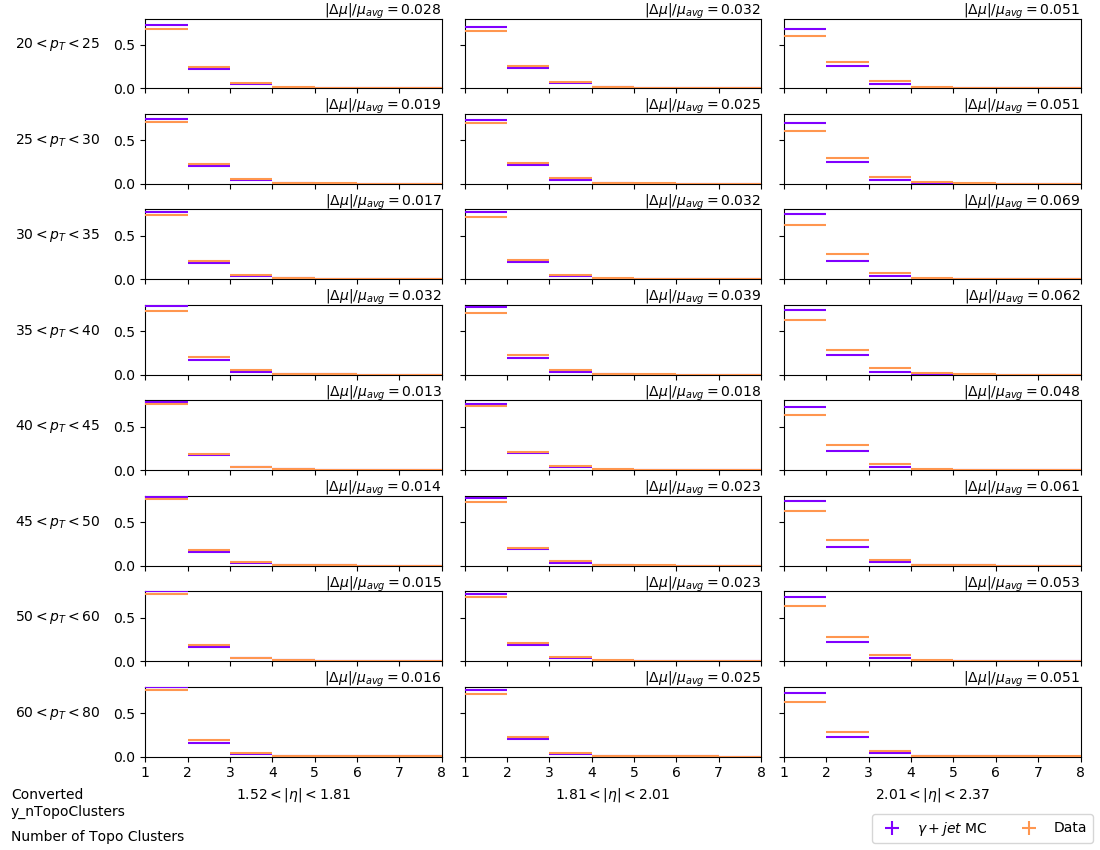
\includegraphics[width=.74\textwidth]{appendices/datamc_images/y_nTopoClusters_Converted_upperEta.png}
    \caption[Data-MC comparison of the number of topo-clusters for converted photons]{Data-MC comparison of the number of topo-clusters for converted photons. The current tight identification is applied to both samples, and the \gls{MC} requires truth-matched photons. The absolute difference of the distribution means normalized to their average mean, $|\Delta \mu|/\mu_{avg}|$ is shown.}
    \label{fig:dmc-c-ntopo}
\end{figure}
\begin{figure}[!thp]
    \centering
    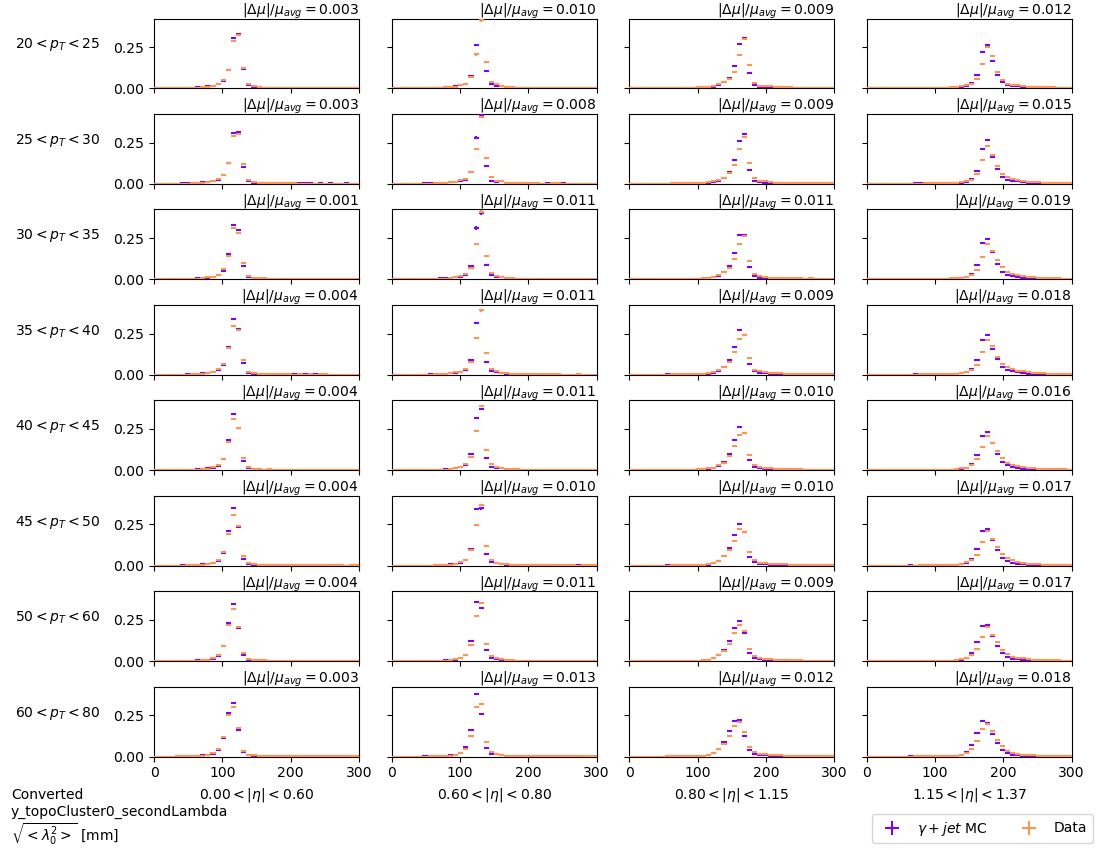
\includegraphics[width=.74\textwidth]{appendices/datamc_images/y_topoCluster0_secondLambda_Converted_lowerEta.png}
    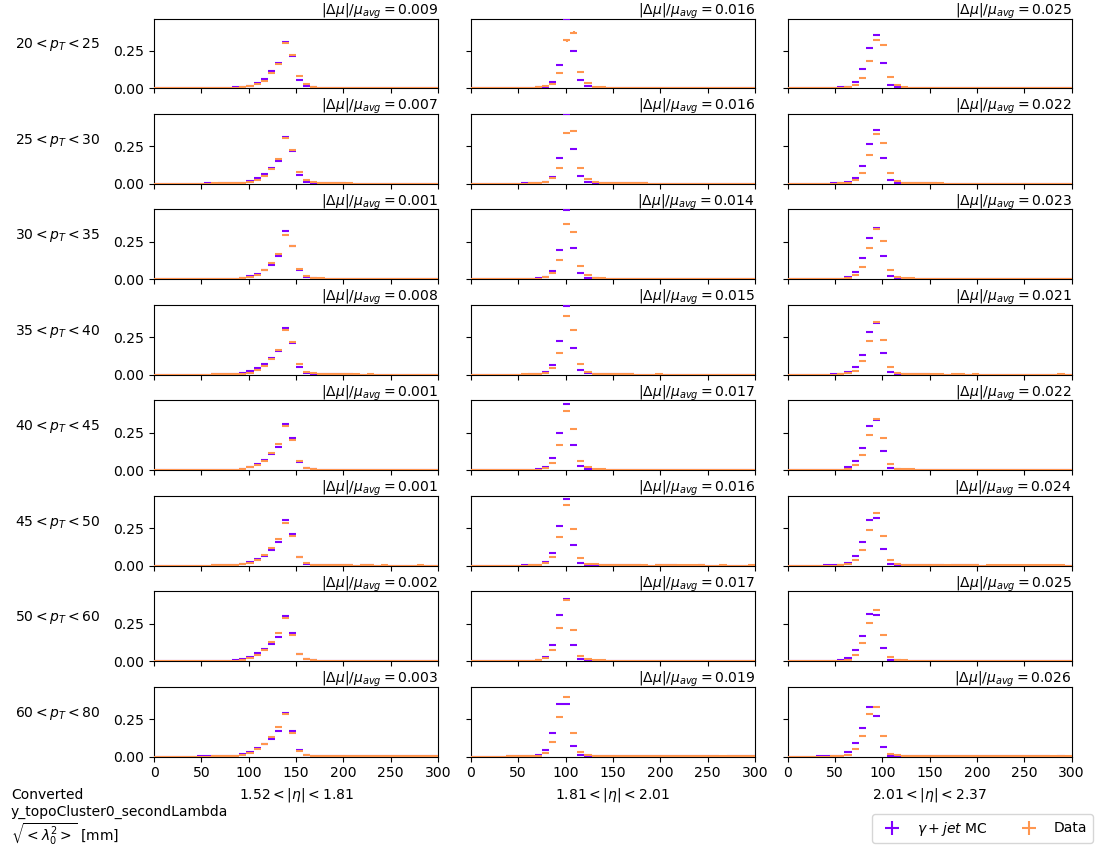
\includegraphics[width=.74\textwidth]{appendices/datamc_images/y_topoCluster0_secondLambda_Converted_upperEta.png}
    \caption[Data-MC comparison of the semi-major axis in depth of the leading topo-cluster (${\sqrt{\lambda_0^2}}$) for converted photons]{Data-MC comparison of the semi-major axis in depth of the leading topo-cluster ($\sqrt{\lambda_0^2}$) for converted photons. The current tight identification is applied to both samples, and the \gls{MC} requires truth-matched photons. The absolute difference of the distribution means normalized to their average mean, $|\Delta \mu|/\mu_{avg}|$ is shown.}
    \label{fig:dmc-c-sl}
\end{figure}
\begin{figure}[!thp]
    \centering
    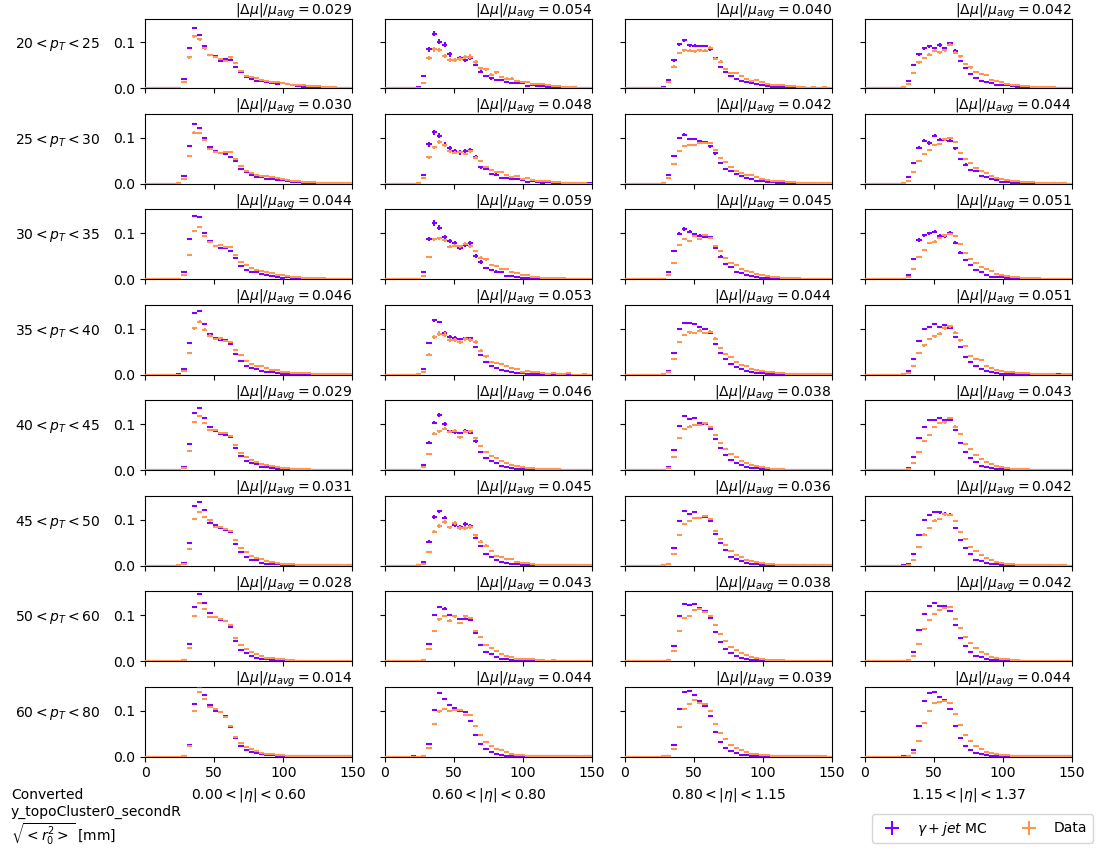
\includegraphics[width=.74\textwidth]{appendices/datamc_images/y_topoCluster0_secondR_Converted_lowerEta.png}
    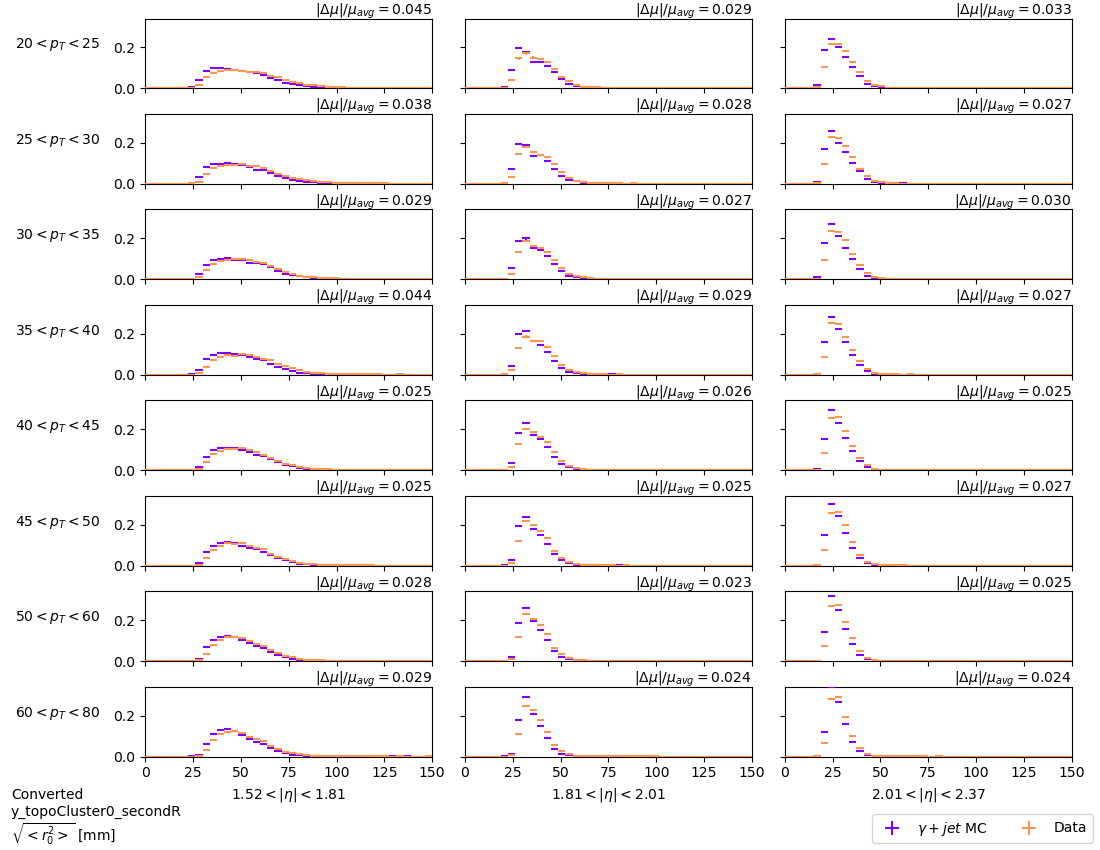
\includegraphics[width=.74\textwidth]{appendices/datamc_images/y_topoCluster0_secondR_Converted_upperEta.png}
    \caption[Data-MC comparison of the semi-major axis in width of the leading topo-cluster ($\sqrt{r_0^2}$) for converted photons]{Data-MC comparison of the semi-major axis in width of the leading topo-cluster ($\sqrt{r_0^2}$) for converted photons.The current tight identification is applied to both samples, and the \gls{MC} requires truth-matched photons. The absolute difference of the distribution means normalized to their average mean, $|\Delta \mu|/\mu_{avg}|$ is shown.}
    \label{fig:dmc-c-sr}
\end{figure}
\begin{figure}[!thp]
    \centering
    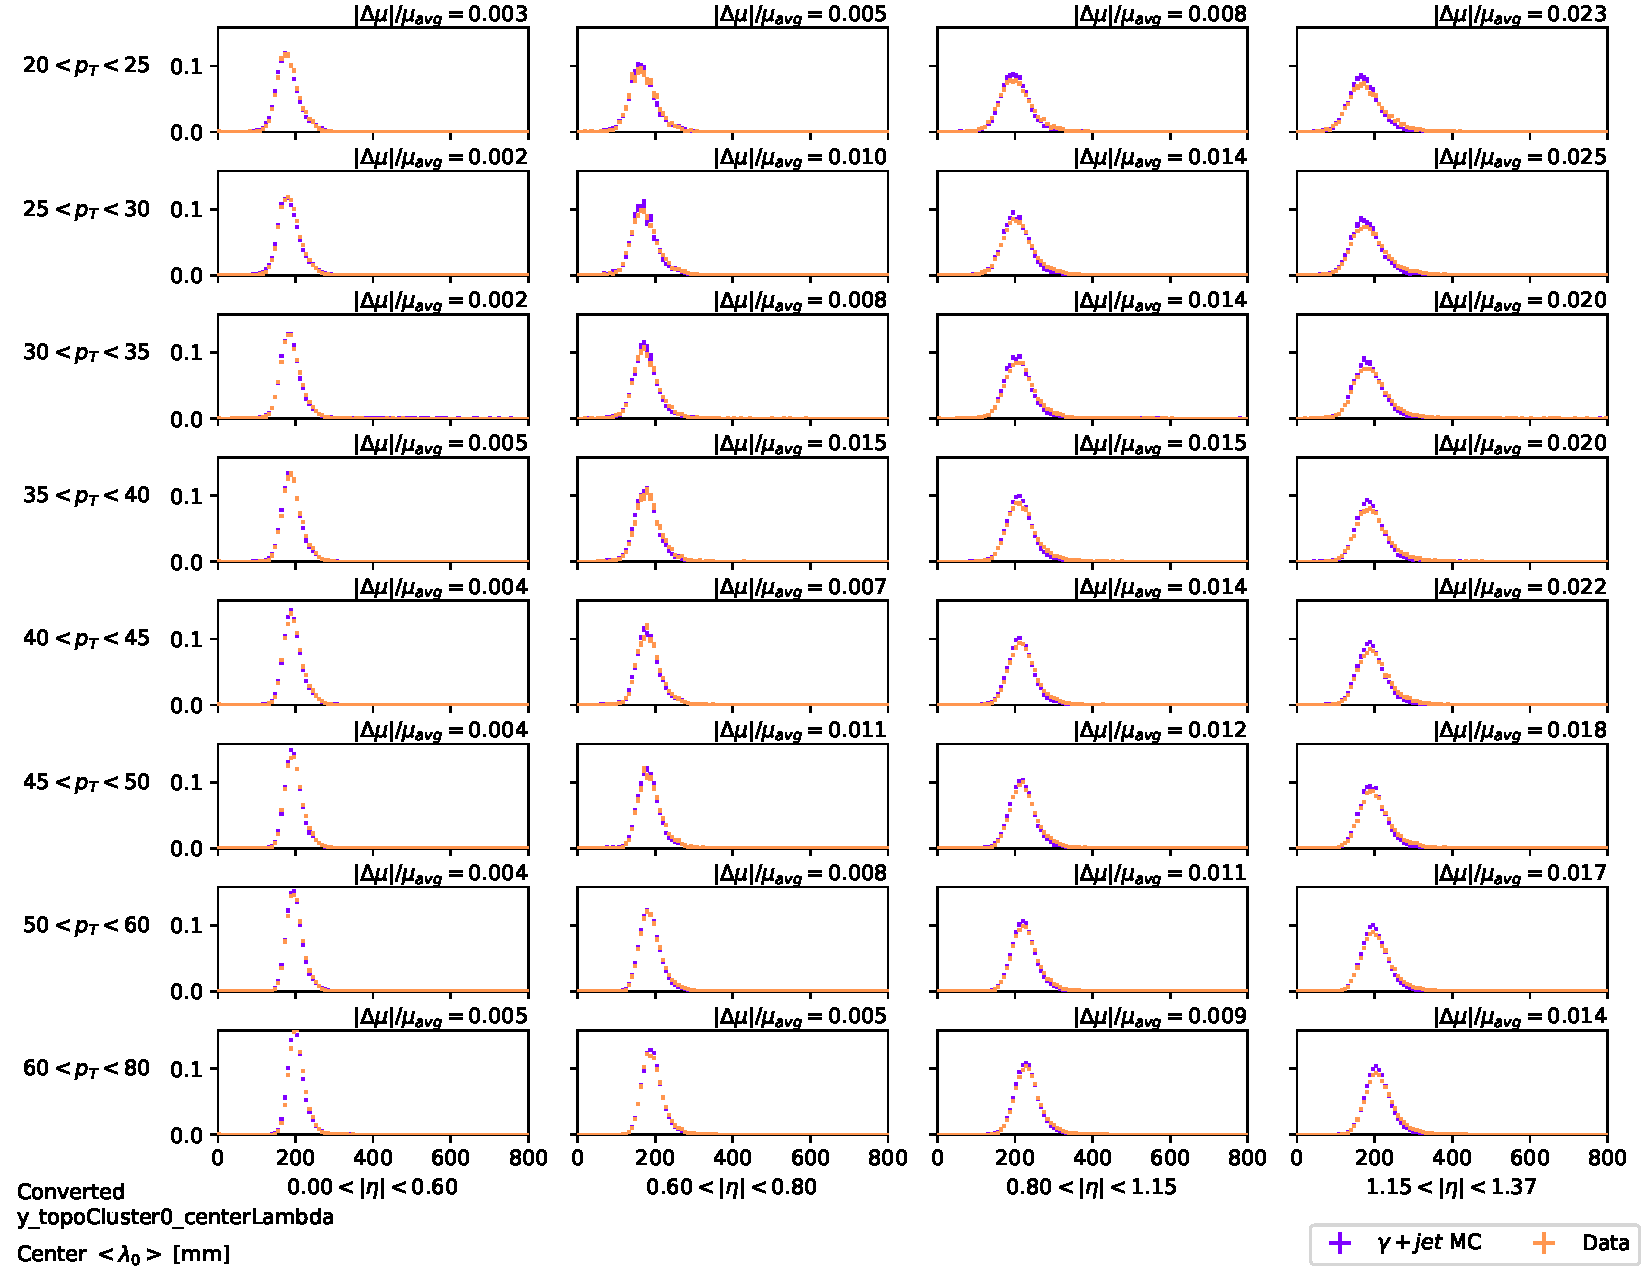
\includegraphics[width=.74\textwidth]{appendices/datamc_images/y_topoCluster0_centerLambda_Converted_lowerEta.pdf}
    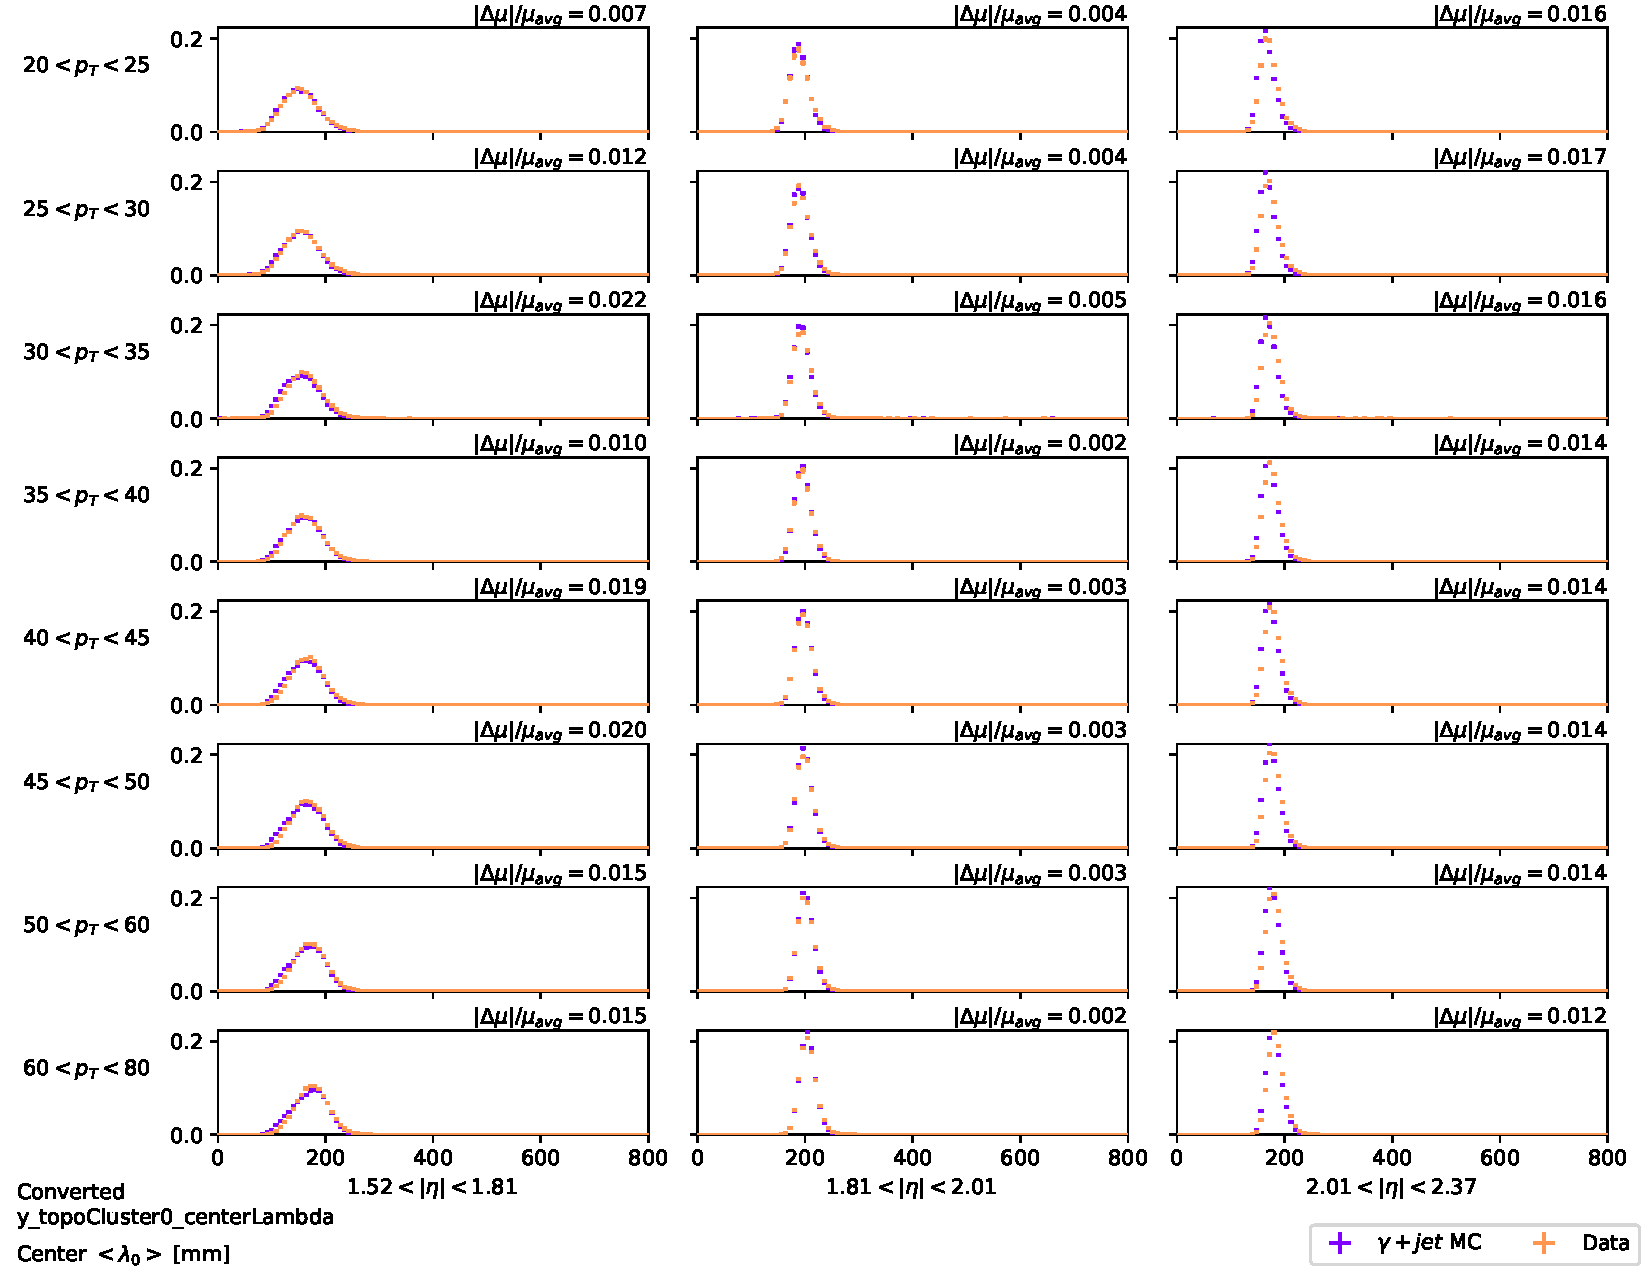
\includegraphics[width=.74\textwidth]{appendices/datamc_images/y_topoCluster0_centerLambda_Converted_upperEta.pdf}
    \caption[Data-MC comparison of the centroid depth of the leading topo-cluster ($<\lambda_{0}>$) for converted photons]{Data-MC comparison of the centroid depth of the leading topo-cluster ($<\lambda_{0}>$) for converted photons. The current tight identification is applied to both samples, and the \gls{MC} requires truth-matched photons. The absolute difference of the distribution means normalized to their average mean, $|\Delta \mu|/\mu_{avg}|$ is shown.}
    \label{fig:dmc-c-cl}
\end{figure}

\begin{figure}[!thp]
    \centering
    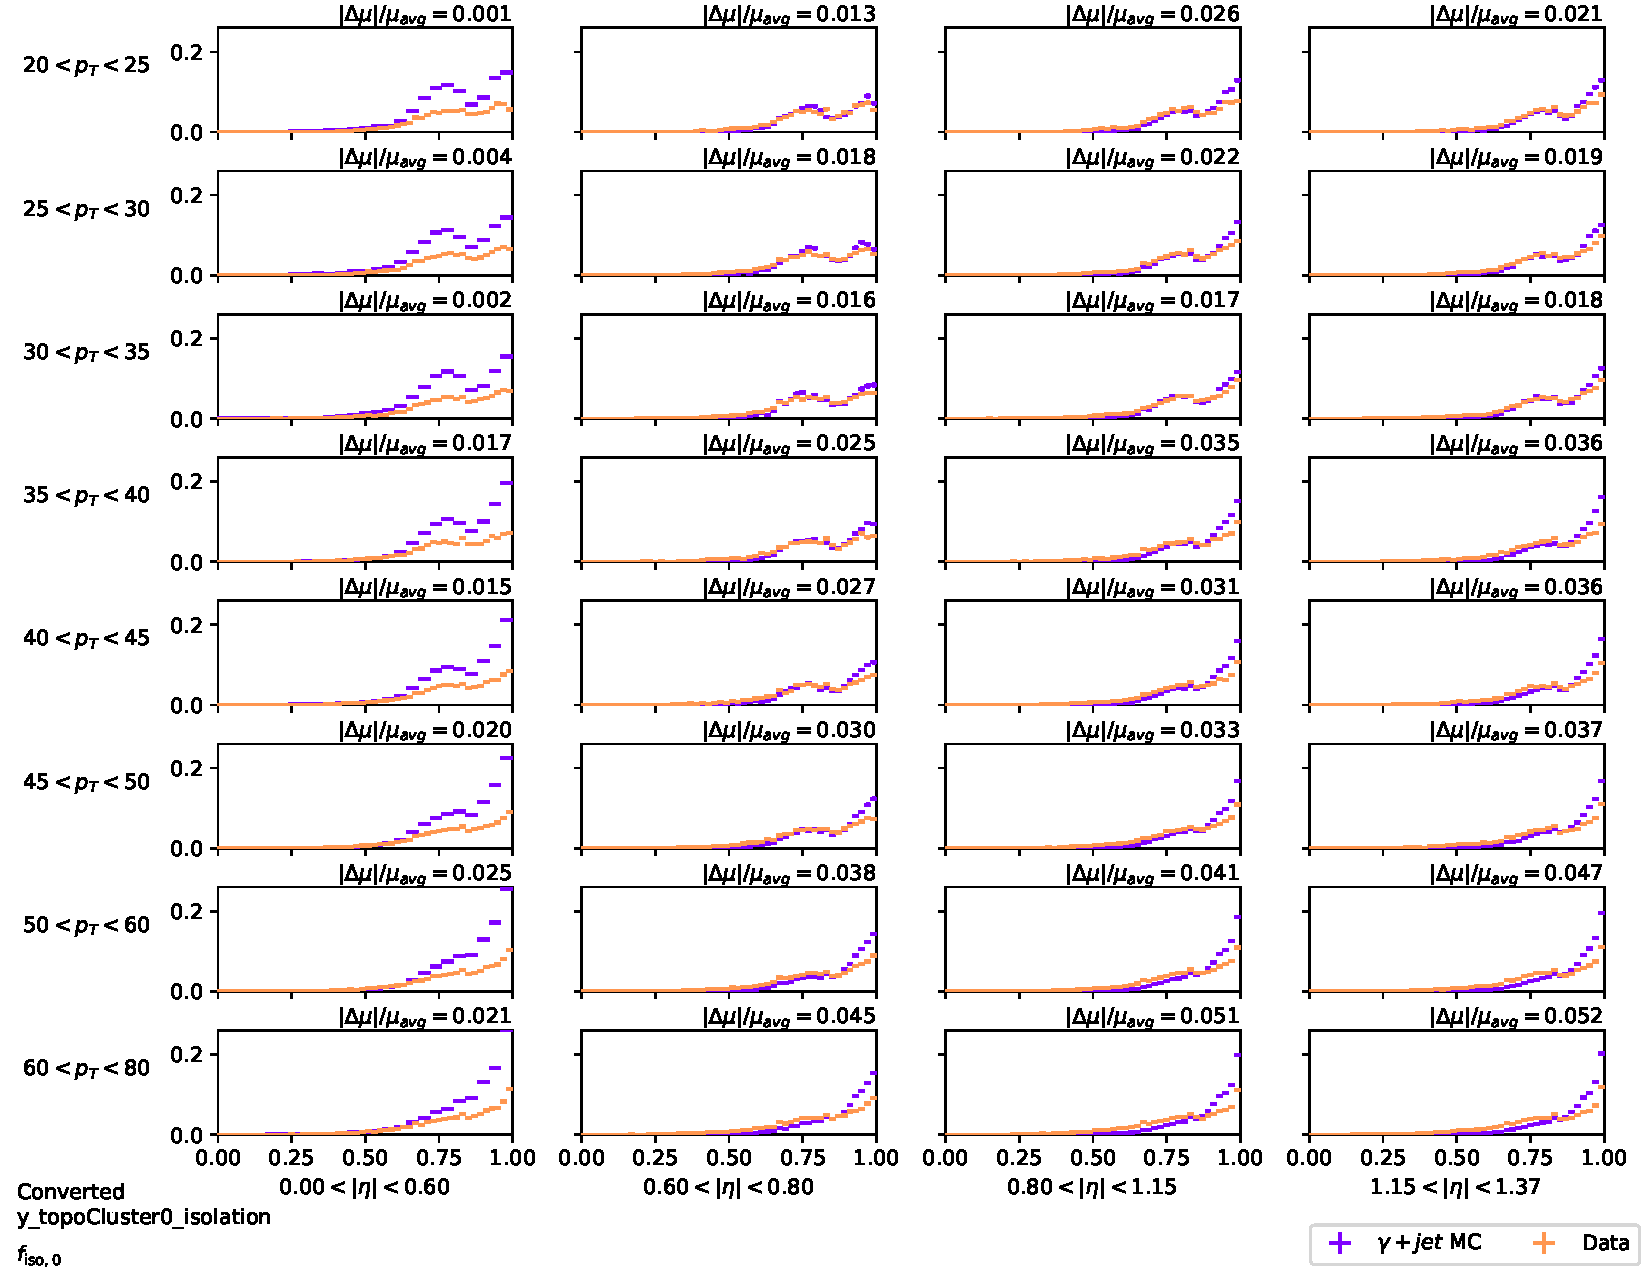
\includegraphics[width=.74\textwidth]{appendices/datamc_images/y_topoCluster0_isolation_Converted_lowerEta.pdf}
    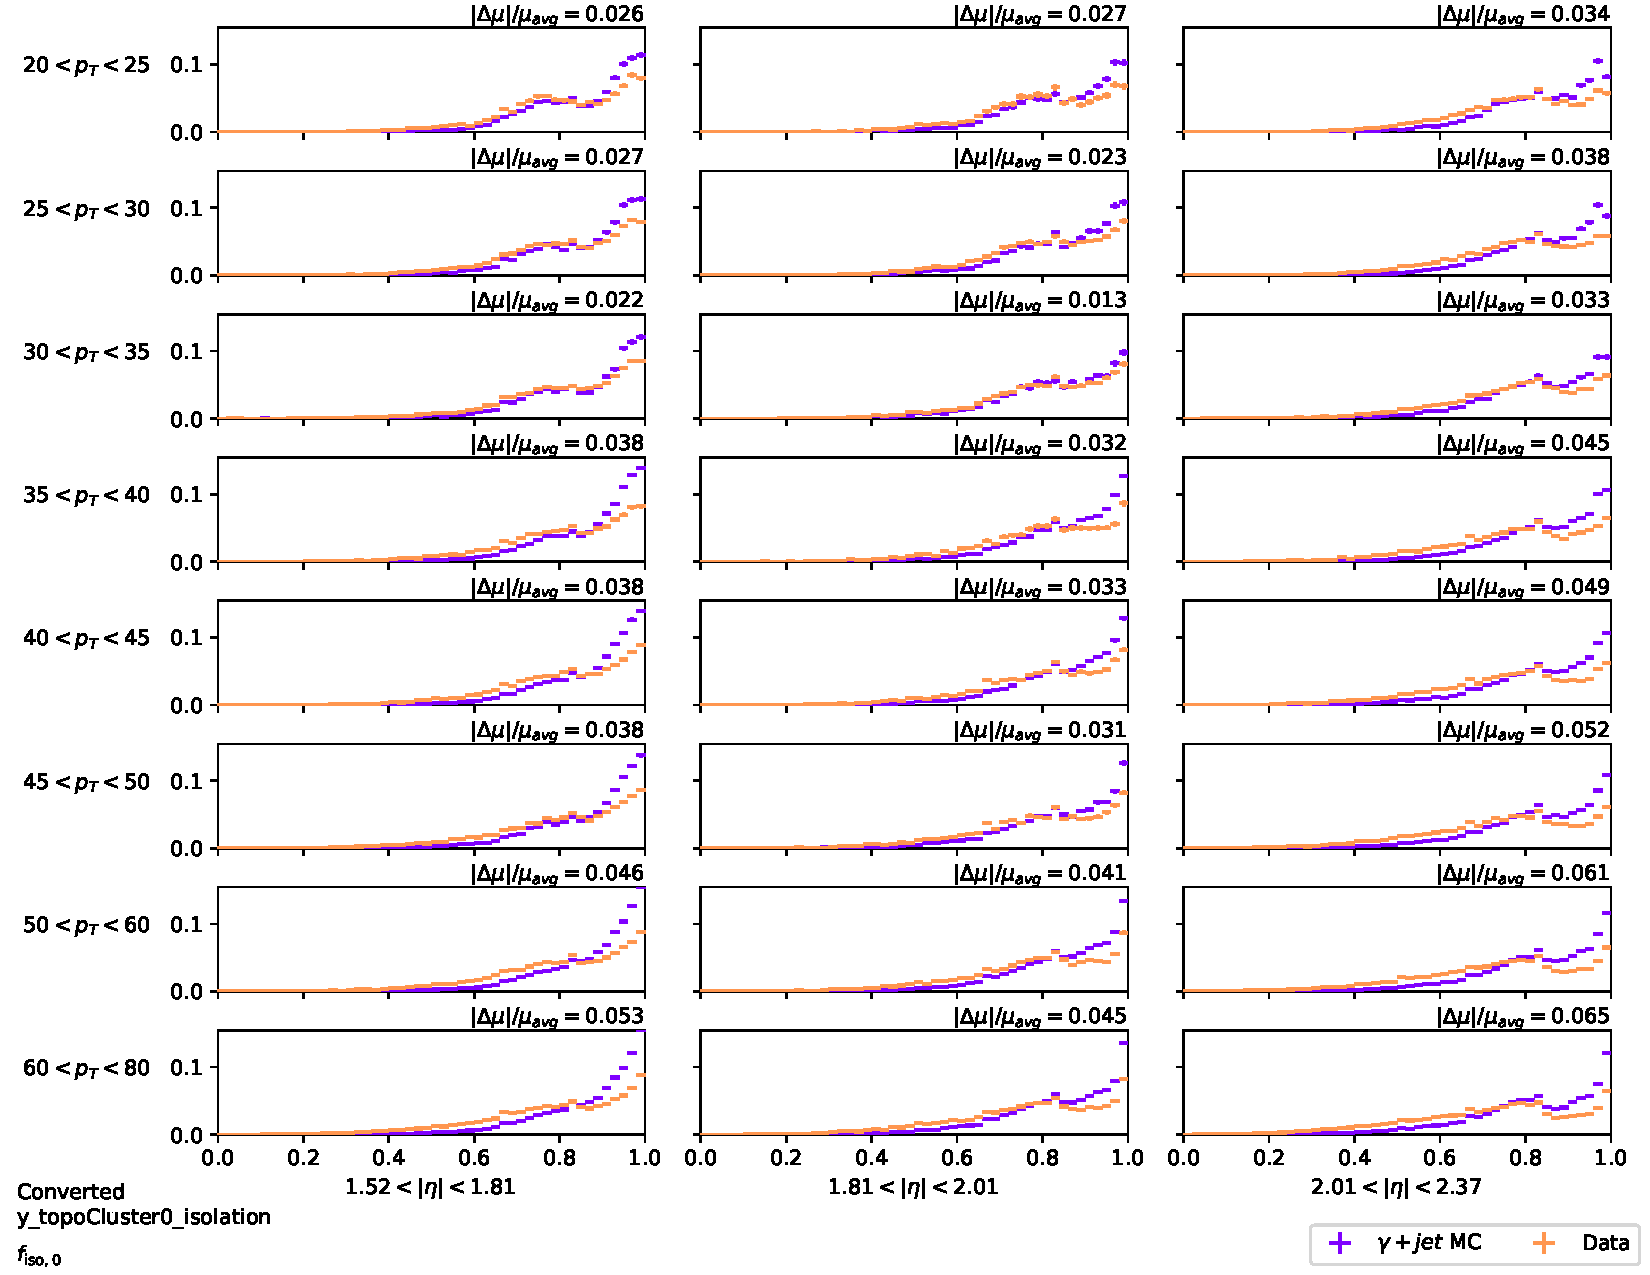
\includegraphics[width=.74\textwidth]{appendices/datamc_images/y_topoCluster0_isolation_Converted_upperEta.pdf}
    \caption[Data-MC comparison of the isolation of the leading topo-cluster ($f_{\text{iso}}$) for converted photons]{Data-MC comparison of the isolation of the leading topo-cluster ($f_{\text{iso}}$) for converted photons. The current tight identification is applied to both samples, and the \gls{MC} requires truth-matched photons. The absolute difference of the distribution means normalized to their average mean, $|\Delta \mu|/\mu_{avg}|$ is shown.}
    \label{fig:dmc-c-iso}
\end{figure}
\begin{figure}[!thp]
    \centering
    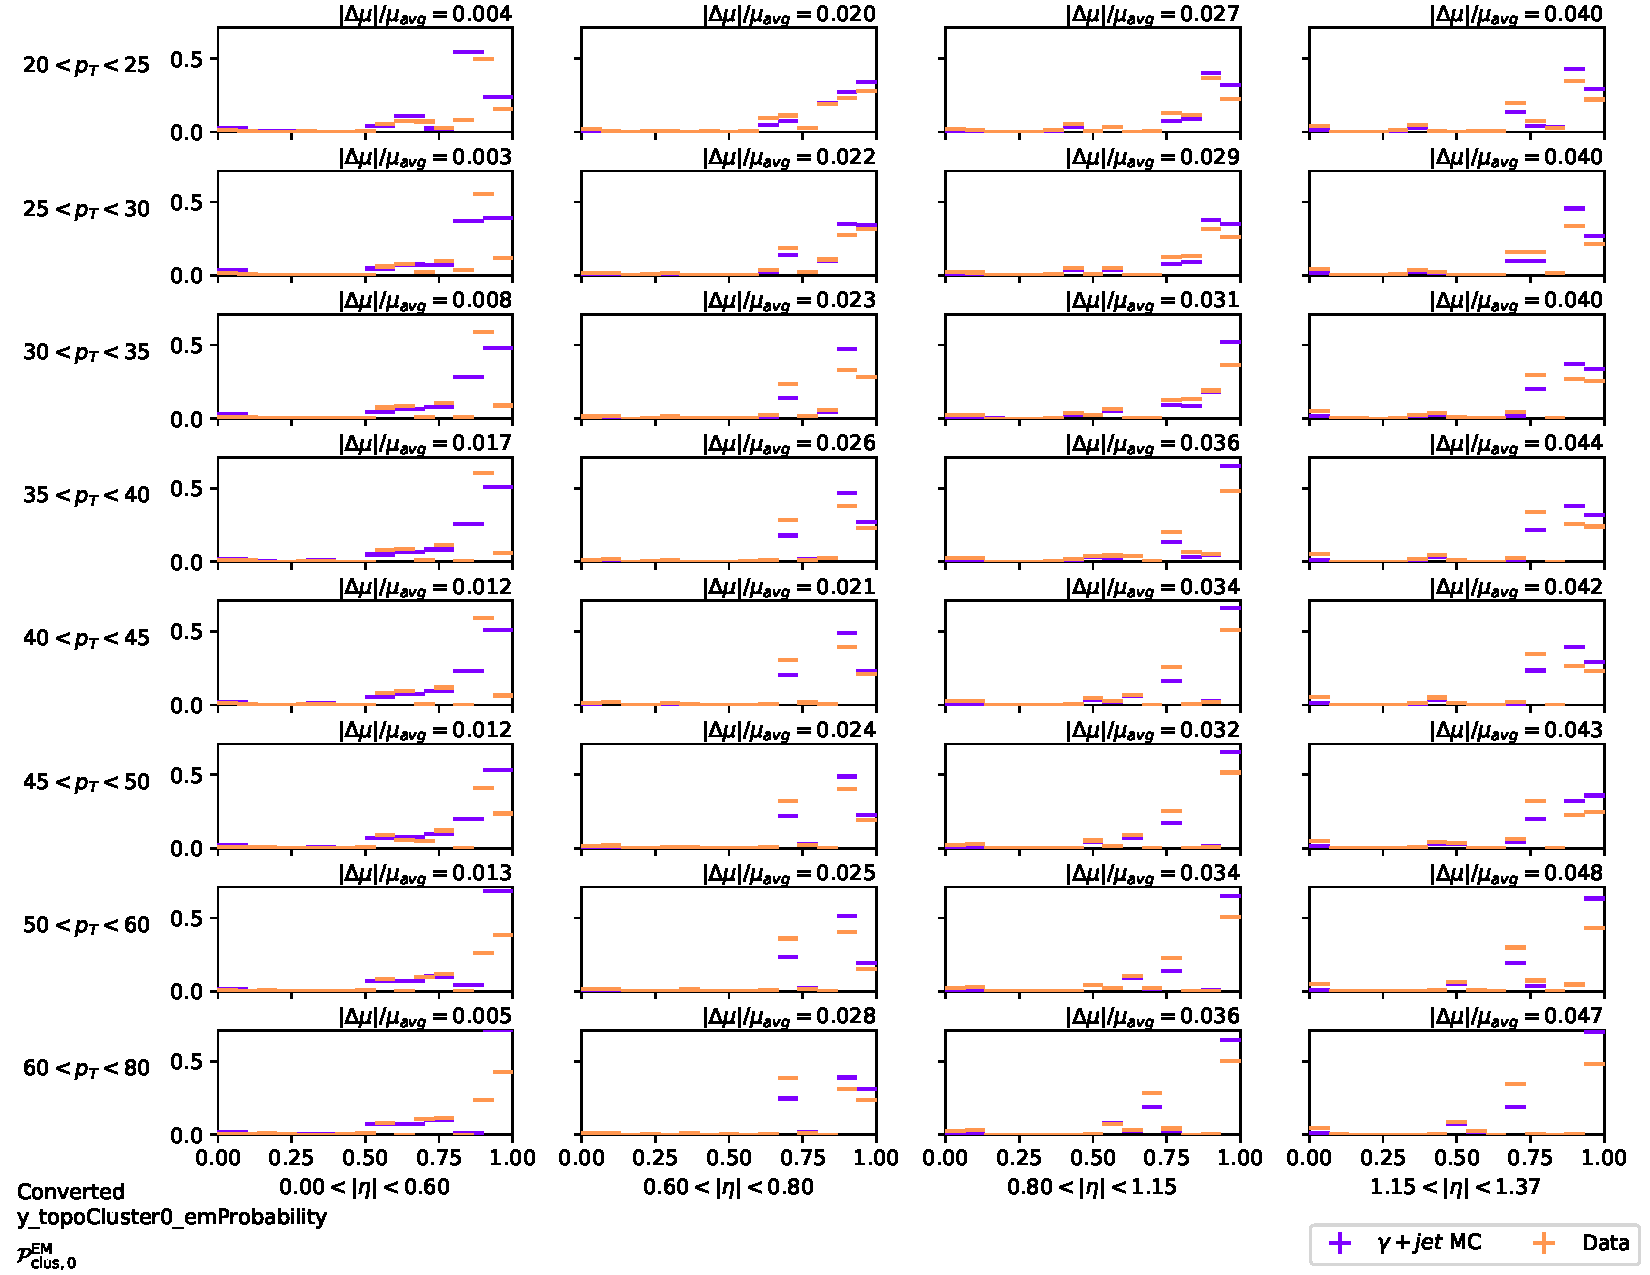
\includegraphics[width=.74\textwidth]{appendices/datamc_images/y_topoCluster0_emProbability_Converted_lowerEta.pdf}
    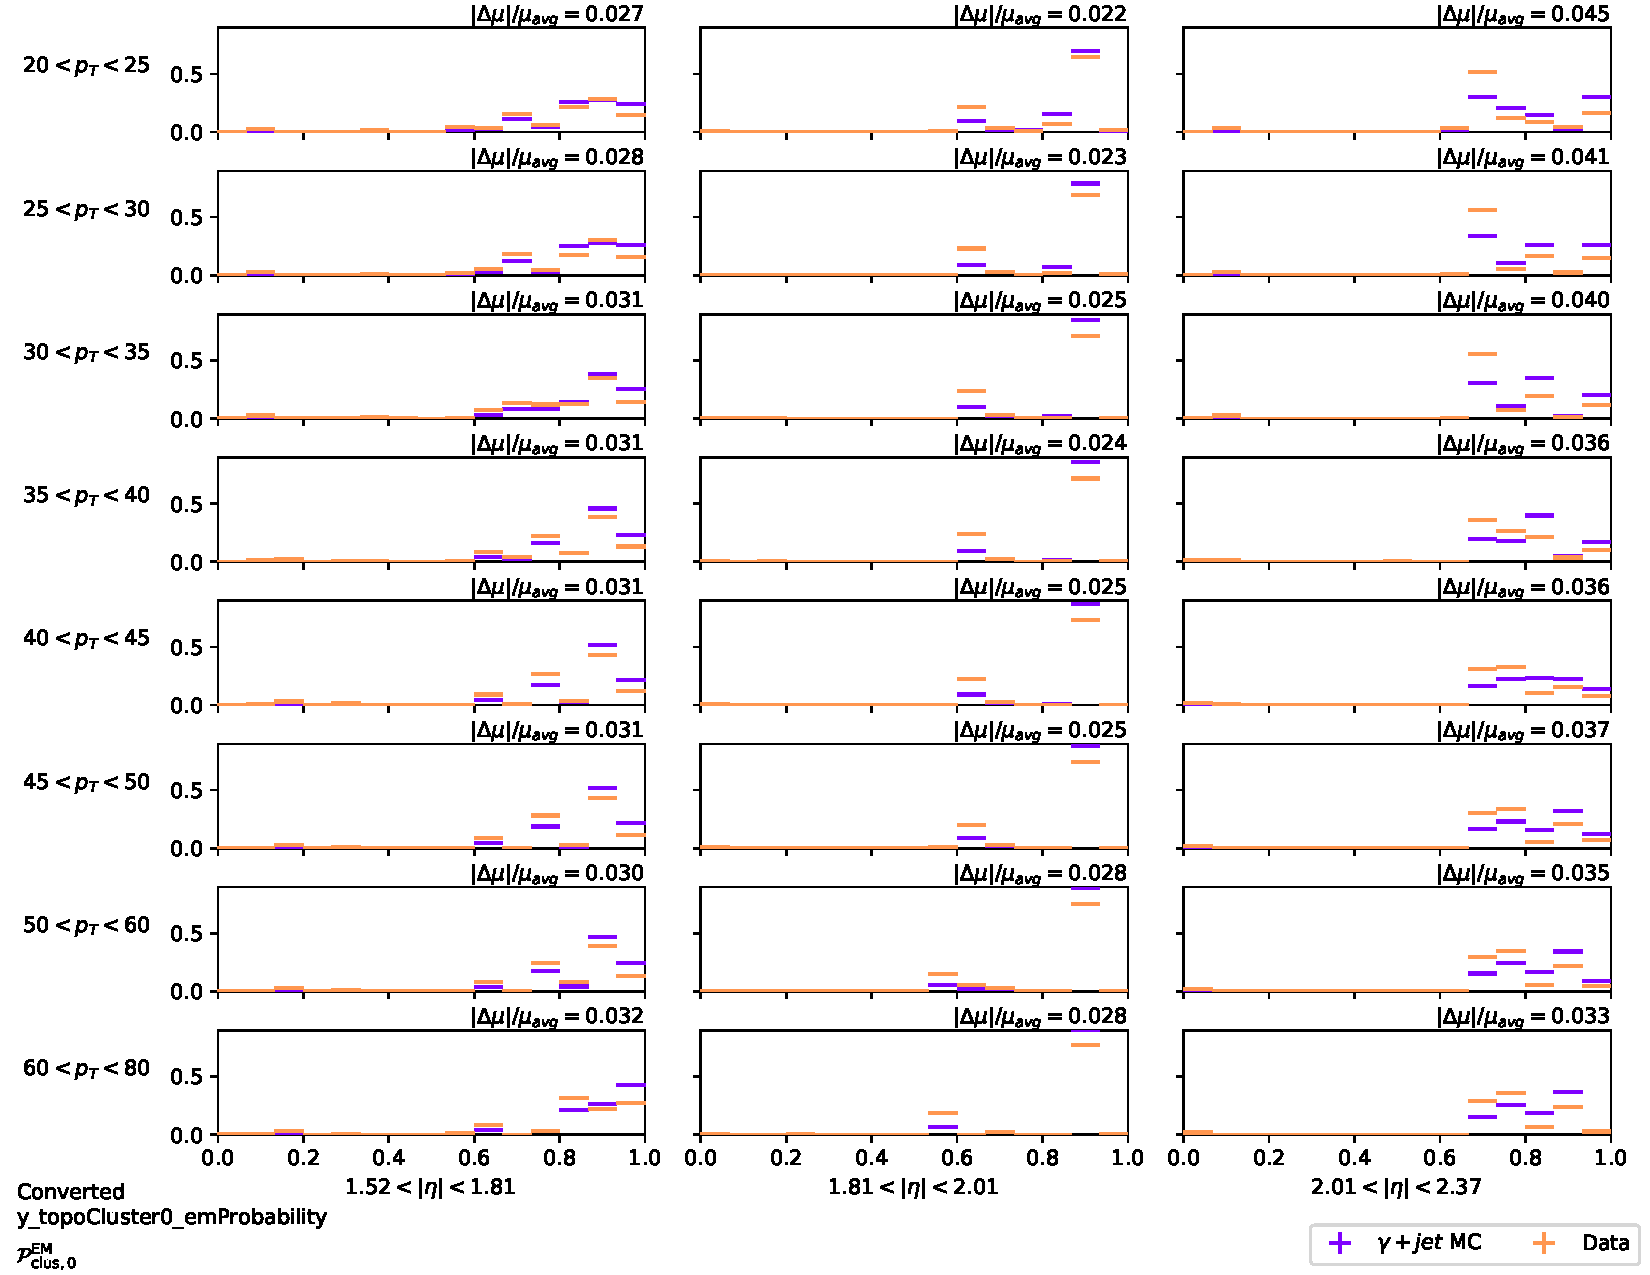
\includegraphics[width=.74\textwidth]{appendices/datamc_images/y_topoCluster0_emProbability_Converted_upperEta.pdf}
    \caption[Data-MC comparison of the \gls{EM} probability of the leading topo-cluster ($\mathcal{P}_{\text{clus}}^{\text{EM}}$) for converted photons]{Data-MC comparison of the \gls{EM} probability of the leading topo-cluster ($\mathcal{P}_{\text{clus}}^{\text{EM}}$) for converted photons. The current tight identification is applied to both samples, and the \gls{MC} requires truth-matched photons. The absolute difference of the distribution means normalized to their average mean, $|\Delta \mu|/\mu_{avg}|$ is shown.}
    \label{fig:dmc-c-emp}
\end{figure}